%%%%%%%%%%%%%%%%%%%%%%%%%%%%%%%%%%%%%%%%%
% Masters/Doctoral Thesis 
% LaTeX Template
% Version 2.5 (27/8/17)
%
% This template was downloaded from:
% http://www.LaTeXTemplates.com
%
% Version 2.x major modifications by:
% Vel (vel@latextemplates.com)
%
% This template is based on a template by:
% Steve Gunn (http://users.ecs.soton.ac.uk/srg/softwaretools/document/templates/)
% Sunil Patel (http://www.sunilpatel.co.uk/thesis-template/)
%
% Template license:
% CC BY-NC-SA 3.0 (http://creativecommons.org/licenses/by-nc-sa/3.0/)
%
%%%%%%%%%%%%%%%%%%%%%%%%%%%%%%%%%%%%%%%%%

%----------------------------------------------------------------------------------------
%	PACKAGES AND OTHER DOCUMENT CONFIGURATIONS
%----------------------------------------------------------------------------------------

\documentclass[
11pt, % The default document font size, options: 10pt, 11pt, 12pt
oneside, % Two side (alternating margins) for binding by default, uncomment to switch to one side
english, % ngerman for German
singlespacing, % Single line spacing, alternatives: onehalfspacing or doublespacing
%draft, % Uncomment to enable draft mode (no pictures, no links, overfull hboxes indicated)
%nolistspacing, % If the document is onehalfspacing or doublespacing, uncomment this to set spacing in lists to single
%liststotoc, % Uncomment to add the list of figures/tables/etc to the table of contents
%toctotoc, % Uncomment to add the main table of contents to the table of contents
parskip, % Uncomment to add space between paragraphs
%nohyperref, % Uncomment to not load the hyperref package
headsepline, % Uncomment to get a line under the header
%chapterinoneline, % Uncomment to place the chapter title next to the number on one line
%consistentlayout, % Uncomment to change the layout of the declaration, abstract and acknowledgements pages to match the default layout
]{MastersDoctoralThesis} % The class file specifying the document structure

\usepackage[utf8]{inputenc} % Required for inputting international characters
\usepackage[T1]{fontenc} % Output font encoding for international characters

\usepackage{mathpazo} % Use the Palatino font by default

\usepackage[backend=bibtex,style=authoryear,natbib=true]{biblatex} % Use the bibtex backend with the authoryear citation style (which resembles APA)

\addbibresource{example.bib} % The filename of the bibliography

\usepackage[autostyle=true]{csquotes} % Required to generate language-dependent quotes in the bibliography

\usepackage{hyperref}
\usepackage{float}

\usepackage{tabu}
\usepackage{glossaries}

\usepackage{listings}
\lstset{
	basicstyle=\small\ttfamily,
	columns=flexible,
	breaklines=true
}

\usepackage{url}

% Generate complete reference using autoref & nameref
\newcommand\gmref[1]{\autoref{#1}~\nameref{#1}}

% Chinese characters
% \usepackage[utf8]{inputenc}
% \usepackage{CJKutf8}
% \newcommand\chn[1]{\begin{CJK}{UTF8}{song}#1\end{CJK}}

% Generate the glossary
\makeglossaries

%----------------------------------------------------------------------------------------
%	MARGIN SETTINGS
%----------------------------------------------------------------------------------------

\geometry{
	paper=a4paper, % Change to letterpaper for US letter
	inner=2.5cm, % Inner margin
	outer=3.8cm, % Outer margin
	bindingoffset=.5cm, % Binding offset
	top=1.5cm, % Top margin
	bottom=1.5cm, % Bottom margin
	%showframe, % Uncomment to show how the type block is set on the page
}

% Maximum nesting numbers. E.g. 1.1.1.1 Section Title
\setcounter{secnumdepth}{3}
% \setcounter{tocdepth}{3}

%----------------------------------------------------------------------------------------
%	THESIS INFORMATION
%----------------------------------------------------------------------------------------

\thesistitle{Development and Comparison of Overview Techniques for Extreme Resolution Datasets} % Your thesis title, this is used in the title and abstract, print it elsewhere with \ttitle
\supervisor{Prof. Dr. Jens \textsc{Krüger}} % Your supervisor's name, this is used in the title page, print it elsewhere with \supname
\examiner{Prof. Dr. Josef \textsc{Pauli}} % Your examiner's name, this is not currently used anywhere in the template, print it elsewhere with \examname
\degree{Bachelor of Science} % Your degree name, this is used in the title page and abstract, print it elsewhere with \degreename
\author{Danyun \textsc{Lei}} % Your name, this is used in the title page and abstract, print it elsewhere with \authorname
\addresses{danyun.lei@stud.uni-due.de} % Your address, this is not currently used anywhere in the template, print it elsewhere with \addressname

\subject{Computer Engineering} % Your subject area, this is not currently used anywhere in the template, print it elsewhere with \subjectname
\keywords{} % Keywords for your thesis, this is not currently used anywhere in the template, print it elsewhere with \keywordnames
\university{\href{https://www.uni-due.com}{Universität Duisburg-Essen}} % Your university's name and URL, this is used in the title page and abstract, print it elsewhere with \univname
\department{\href{https://www.uni-due.de/ise/}{International Studies in Engineering (ISE) PO08}} % Your department's name and URL, this is used in the title page and abstract, print it elsewhere with \deptname
\group{\href{https://www.uni-due.de/ise/}{Computer Engineering}} % Your research group's name and URL, this is used in the title page, print it elsewhere with \groupname
\faculty{\href{https://www.uni-due.de/iw/}{Fakultät für Ingenieurwissenschaften}} % Your faculty's name and URL, this is used in the title page and abstract, print it elsewhere with \facname

\AtBeginDocument{
\hypersetup{pdftitle=\ttitle} % Set the PDF's title to your title
\hypersetup{pdfauthor=\authorname} % Set the PDF's author to your name
\hypersetup{pdfkeywords=\keywordnames} % Set the PDF's keywords to your keywords
}

\usepackage{nameref}
\usepackage{cleveref}

\begin{document}

\frontmatter % Use roman page numbering style (i, ii, iii, iv...) for the pre-content pages

\pagestyle{plain} % Default to the plain heading style until the thesis style is called for the body content

%----------------------------------------------------------------------------------------
%	TITLE PAGE
%----------------------------------------------------------------------------------------

\begin{titlepage}
\begin{center}

\vspace*{.01\textheight}
{\scshape\LARGE \univname\par}\vspace{1.5cm} % University name
\textsc{\Large Bachelor Thesis}\\[0.5cm] % Thesis type

\HRule \\[0.4cm] % Horizontal line
{\huge \bfseries \ttitle\par}\vspace{0.4cm} % Thesis title
\HRule \\[1cm] % Horizontal line
 
\begin{minipage}[t]{0.4\textwidth}
\begin{flushleft} \large
\emph{Author:}\\
\href{http://www.uni-due.de}{\authorname} % Author name - remove the \href bracket to remove the link
\end{flushleft}
\end{minipage}
\begin{minipage}[t]{0.4\textwidth}
\begin{flushright} \large
\emph{Supervisor:} \\
\href{http://www.uni-due.de}{\supname} % Supervisor name - remove the \href bracket to remove the link  
\end{flushright}
\end{minipage}\\[0.4cm]

\begin{minipage}[t]{0.4\textwidth}
\begin{flushleft} \large
\end{flushleft}
\end{minipage}
\begin{minipage}[t]{0.4\textwidth}
\begin{flushright} \large
\emph{Examiners:} \\
\href{http://www.uni-due.de}{\supname} \\
\href{http://www.uni-due.de}{\examname} \\ % Supervisor name - remove the \href bracket to remove the link  
\end{flushright}
\end{minipage}\\[1.7cm]
 
% \vfill

\footnotesize \textit{A thesis submitted in fulfillment of the requirements\\ for the degree of \degreename}\\[0.3cm] % University requirement text
\textit{in}\\[0.4cm]
\large Computer Engineering\\
International Studies in Engineering (ISE) PO08\\
Fakultät für Ingenieurwissenschaften\\[0.5cm] % Research group name and department name
\footnotesize \textit{for}\\[0.4cm]
\large The High Performance Computing Group\\
Department Engineering\\[2cm] % Research group name and department name
 
% \vfill

{\large \today}\\[4cm] % Date
%\includegraphics{Logo} % University/department logo - uncomment to place it
 
\vfill
\end{center}
\end{titlepage}

%----------------------------------------------------------------------------------------
%	DECLARATION PAGE
%----------------------------------------------------------------------------------------
\begin{declaration}
\addchaptertocentry{\authorshipname} % Add the declaration to the table of contents
% \noindent I, \authorname, declare that this thesis titled, \enquote{\ttitle} and the work presented in it are my own. I confirm that:

% \begin{itemize} 
% \item This work was done wholly or mainly while in candidature for a research degree at this University.
% \item Where any part of this thesis has previously been submitted for a degree or any other qualification at this University or any other institution, this has been clearly stated.
% \item Where I have consulted the published work of others, this is always clearly attributed.
% \item Where I have quoted from the work of others, the source is always given. With the exception of such quotations, this thesis is entirely my own work.
% \item I have acknowledged all main sources of help.
% \item Where the thesis is based on work done by myself jointly with others, I have made clear exactly what was done by others and what I have contributed myself.\\
% \end{itemize}
 
% \noindent Signed:\\
% \rule[0.5em]{25em}{0.5pt} % This prints a line for the signature
 
% \noindent Date:\\
% \rule[0.5em]{25em}{0.5pt} % This prints a line to write the date

\noindent Ich, \authorname, versichere an Eides statt durch meine untenstehende Unterschrift,

\begin{itemize} 
\item dass ich die vorliegende Arbeit - mit Ausnahme der Anleitung durch die Betreuer - selbstst\"andig ohne fremde Hilfe angefertigt habe und
\item dass ich alle Stellen, die w\"ortlich oder ann\"ahernd w\"ortlich aus fremden Quellen entnommen sind, entsprechend als Zitate gekennzeichnet habe und
\item dass ich ausschließlich die angegebenen Quellen (Literatur, Internetseiten, sonstige Hilfsmittel) verwendet habe und
\item dass ich alle entsprechenden Angaben nach bestem Wissen und Gewissen vorgenommen habe, dass sie der Wahrheit entsprechen und dass ich nichts verschwiegen habe.
\end{itemize}

\noindent Mir ist bekannt, dass eine falsche Versicherung an Eides Statt nach \S 156 und nach \S 163 Abs. 1 des Strafgesetzbuches mit Freiheitsstrafe oder Geldstrafe bestraft wird.\\[.4cm]

% Ort, Datum
% Unterschrift

\begin{center}
	\begin{tabu} to .95\textwidth { X[l] X[c] X[r] }
		~ & ~ & ~ \\
		\cline{1-1} \cline{3-3} \\
		Ort, Datum  & ~  & Unterschrift \\
	\end{tabu}
\end{center}

\end{declaration}

\cleardoublepage

%----------------------------------------------------------------------------------------
%	QUOTATION PAGE
%----------------------------------------------------------------------------------------

\vspace*{0.2\textheight}

\noindent\enquote{\itshape To see a world in a grain of sand, hold infinity in the palm of your hand. }\bigbreak

\hfill William Blake

%----------------------------------------------------------------------------------------
%	ABSTRACT PAGE
%----------------------------------------------------------------------------------------

\begin{abstract}
\addchaptertocentry{\abstractname} % Add the abstract to the table of contents

% 本文以Mandelbrot数据集为例,开发、实现了三种主要的总览技术以及两种辅助性的(Secondary)总览的预览效果,对于极高分辨率的数据集,采用了层次结构来呈现数据集信息,通过开发的程序可以很直观地理解所观察的数据集对于整体来说所处于的位置的层级状态,并对组合成的总览技术方式进行了比较。值得一提的是本文所实现的Mandelbrot数据集,对于极高分辨率数据集一个非常好的例子,因为它是一个可以在理论上提供无限高的分辨率的数据集。本文所使用的技术为纯web技术,是html/js/css的经典组合,并提供了将纯前端技术替换为前后端分离的可能性。

In this thesis, three main overview techniques and two secondary preview techniques of the overviews are developed and implemented using the Mandelbrot set as the source of extreme resolution datasets. For these datasets, a hierarchical structure is used to present the index information of the current region of interest. Using the developed software in this thesis, it is possible to intuitively understand the hierarchical state of the current observing area with the whole. This thesis also compares the different overview techniques which in combination consists of six different ways.

\noindent It is worth mentioning that the Mandelbrot set that are implemented in this thesis is a very good example for extreme high resolution datasets because it is a dataset that can theoretically provide infinitely high resolution.

\noindent The technology stack used in this thesis is pure web technology, a classic combination of \texttt{HTML} / \texttt{JavaScript} / \texttt{CSS}, and the program offers the possibility to adapt and replace the pure front-end technology with front and back end separation solution easily.

\end{abstract}

%----------------------------------------------------------------------------------------
%	ACKNOWLEDGEMENTS
%----------------------------------------------------------------------------------------

\begin{acknowledgements}
\addchaptertocentry{\acknowledgementname} % Add the acknowledgements to the table of contents
% The acknowledgments and the people to thank go here, don't forget to include your project advisor\ldots
I hereby express my deep sense of gratitude and indebtedness to Prof. Dr. Jens Krüger, for your valuable guidance, encouragement and support. Your patience and faith in me was a key reason that I could finish the work.

\noindent Also I express my thanks to Prof. Dr. Yunqi Lei, Dr. Bixia Wu and Dr. Franz-Josef Schmitz, in no particular order. Without your support, I could not have finished the task successfully.
\end{acknowledgements}

%----------------------------------------------------------------------------------------
%	LIST OF CONTENTS/FIGURES/TABLES PAGES
%----------------------------------------------------------------------------------------

{
	\hypersetup{linkcolor = red!40!black}
	\tableofcontents % Prints the main table of contents
}

{
	\hypersetup{linkcolor = red!30!black}
	\listoffigures % Prints the list of figures
}

{
	\hypersetup{linkcolor = red!25!black}
	\listoftables % Prints the list of tables
}

%----------------------------------------------------------------------------------------
%	ABBREVIATIONS
%----------------------------------------------------------------------------------------

\begin{abbreviations}{ll} % Include a list of abbreviations (a table of two columns)

\textbf{HTML}\label{glo:html} & \textbf{H}ypertext \textbf{M}arkup \textbf{L}anguage\\
\textbf{JS}\label{glo:js} & \textbf{J}ava\textbf{S}cript\\
\textbf{CSS}\label{glo:css} & \textbf{C}ascading \textbf{S}tyle \textbf{S}heets\\
\textbf{DOM}\label{glo:dom} & \textbf{D}ocument \textbf{O}bject \textbf{M}odel\\
\textbf{URL}\label{glo:url} & \textbf{U}niform \textbf{R}esource \textbf{L}ocator\\
\textbf{JSON}\label{glo:json} & \textbf{J}ava \textbf{S}cript \textbf{O}bject \textbf{N}otation\\
\textbf{UI}\label{glo:ui} & \textbf{U}ser \textbf{I}nterface\\

\newglossaryentry{html}{name = {HTML}, description = {Hypertext Markup Language}}
\newglossaryentry{js}{name = {JS}, description = {JavaScript}}
\newglossaryentry{css}{name = {CSS}, description = {Cascading Style Sheets}}
\newglossaryentry{dom}{name = {DOM}, description = {Document Object Model}}
\newglossaryentry{url}{name = {URL}, description = {Uniform Resource Locator}}
\newglossaryentry{json}{name = {JSON}, description = {Java Script Object Notation}}
\newglossaryentry{ui}{name = {UI}, description = {User Interface}}

\end{abbreviations}

%----------------------------------------------------------------------------------------
%	PHYSICAL CONSTANTS/OTHER DEFINITIONS
%----------------------------------------------------------------------------------------

\begin{constants}{lr@{${}={}$}l} % The list of physical constants is a three column table

% The \SI{}{} command is provided by the siunitx package, see its documentation for instructions on how to use it

Speed of Light & $c_{0}$ & \SI{2.99792458e8}{\meter\per\second} (exact)\\
%Constant Name & $Symbol$ & $Constant Value$ with units\\

\end{constants}

%----------------------------------------------------------------------------------------
%	SYMBOLS
%----------------------------------------------------------------------------------------

\begin{symbols}{lll} % Include a list of Symbols (a three column table)

$a$ & distance & \si{\meter} \\
$P$ & power & \si{\watt} (\si{\joule\per\second}) \\
%Symbol & Name & Unit \\

\addlinespace % Gap to separate the Roman symbols from the Greek

$\omega$ & angular frequency & \si{\radian} \\

\end{symbols}

%----------------------------------------------------------------------------------------
%	DEDICATION
%----------------------------------------------------------------------------------------

\dedicatory{Special thanks to Dr. Zhonghua Xu, Ms. Meng Wang and Mrs. Vivian E. Rice, I wish I could share the joy of this achievements with all of you - here or in Azeroth.} 

%----------------------------------------------------------------------------------------
%	THESIS CONTENT - CHAPTERS
%----------------------------------------------------------------------------------------

\mainmatter % Begin numeric (1,2,3...) page numbering

\pagestyle{thesis} % Return the page headers back to the "thesis" style

% Include the chapters of the thesis as separate files from the Chapters folder
% Uncomment the lines as you write the chapters

% Set hyperlink color
\hypersetup{linkcolor = red!45!black}

% Chapter Template

\chapter{Introduction and Motivation} % Main chapter title

\label{Chapter1} % Change X to a consecutive number; for referencing this chapter elsewhere, use \ref{ChapterX}

%----------------------------------------------------------------------------------------
%	SECTION
%----------------------------------------------------------------------------------------

\section{Introduction}

In many modern-day applications and computer programs, we may encounter frequently a situation where users have to browse or interact with a large set of data or information, however, only focusing only on a certain part of them. In many situations, this part is usually a lot smaller than the original dataset relatively. The most commonly seen scenario would be a \gls{gis} programs on computers, for example an \gls{opd} display as shown in \gmref{fig:usgsmap}. These type of applications usually have a zoomable interface to allow users to zoom into a specific region of the original dataset. Also they usually allow users to browse around the dataset from the current focus region and navigate and interact with the whole large dataset with the sense of the ``large picture'' by the mechanism of \gls{opd} techniques.

\begin{figure}[th]
\centering
% 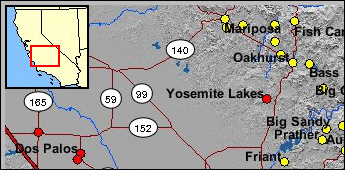
\includegraphics[width=\textwidth,keepaspectratio]{Figures/Chapter1/usgsmap.png}
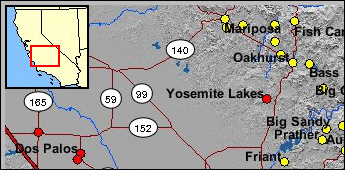
\includegraphics{Figures/Chapter1/usgsmap.png}
\decoRule
\caption[Overview Plus Detail on Map]{From \url{http://wildfire.usgs.gov}, an overview of the graphics next to a zoomed ``detail view''.}
\label{fig:usgsmap}
\end{figure}

Other examples besides \gls{gis} include also some image processing and image generation applications such as Photoshop shown in \gmref{fig:ps}, because usually the resolution of the image being processed or generated is larger than the resolution of one single screen monitor. Another interesting example would be in the modern computer gaming industry, that the concept of \emph{Mini-map}s were invented, illustrated in \gmref{fig:minimap}, with the same concepts due to the fact that the virtual world of digital games is mostly a lot larger than how much one single screen can contain.

\begin{figure}[th]
\centering
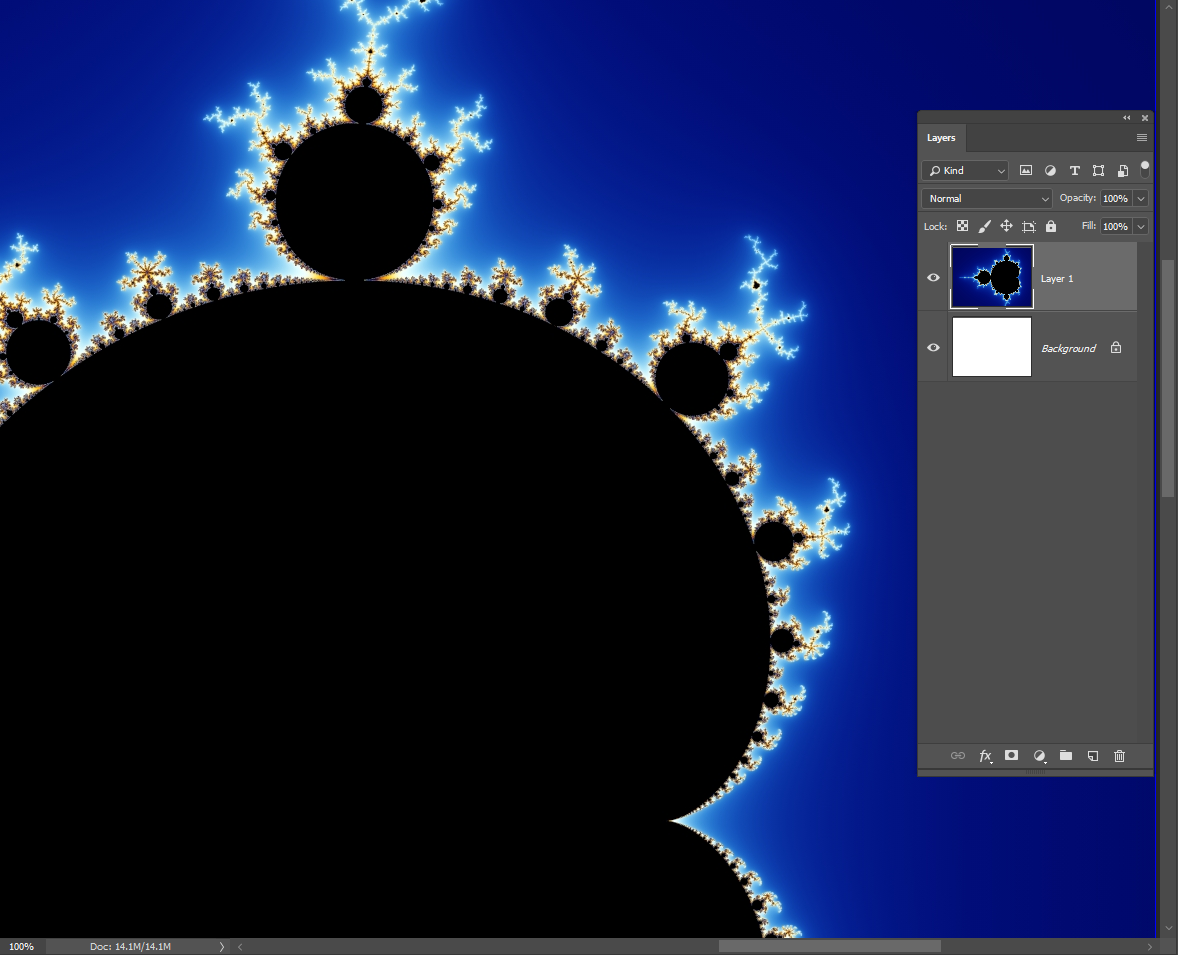
\includegraphics[width=\textwidth,keepaspectratio]{Figures/Chapter1/ps.png}
% 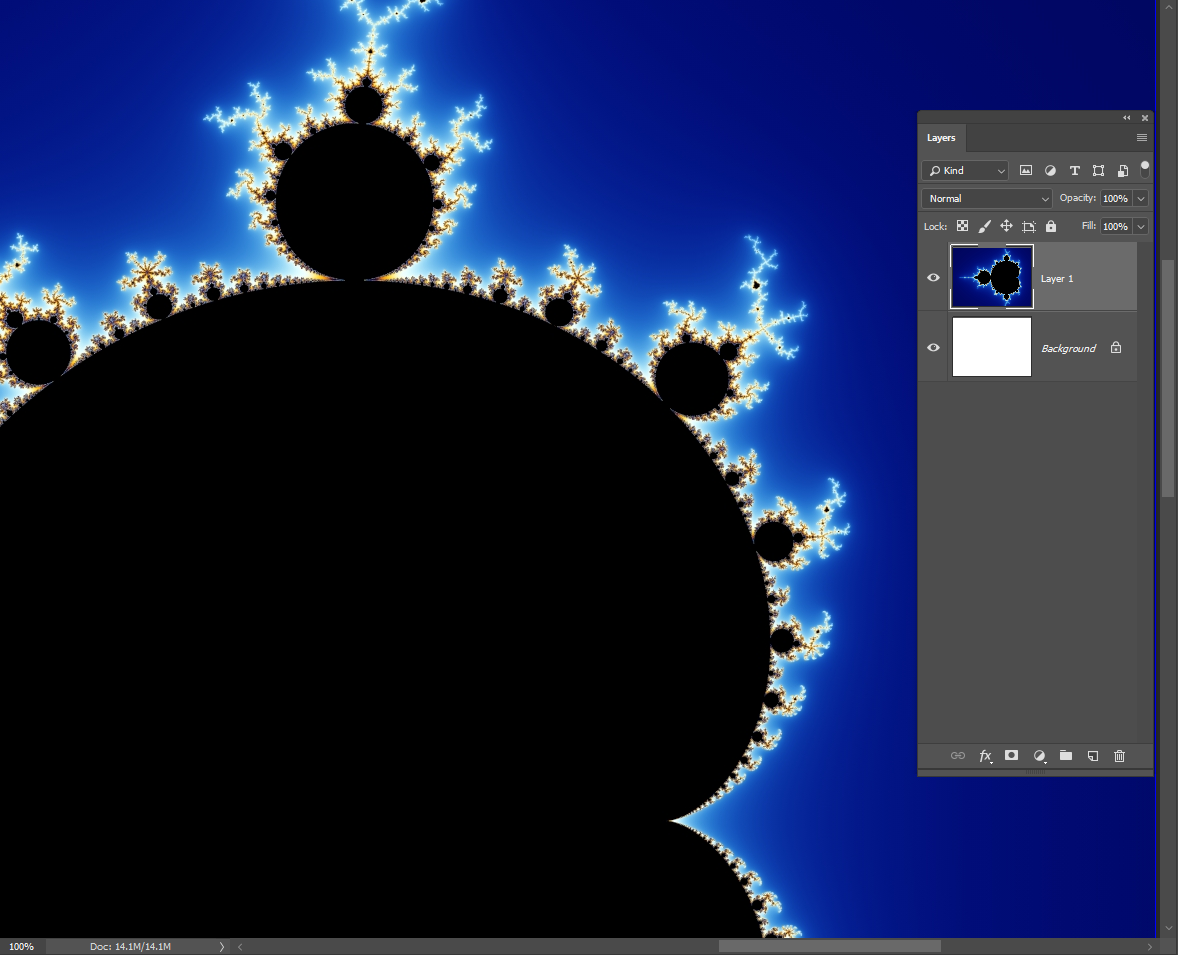
\includegraphics{Figures/Chapter1/ps.png}
\decoRule
\caption[Overview Plus Detail in Photoshop]{The basic mechanism in the application Photoshop, layers, offering an overview functionality, with detailed focus area on the main visual area.}
\label{fig:ps}
\end{figure}

\begin{figure}[th]
\centering
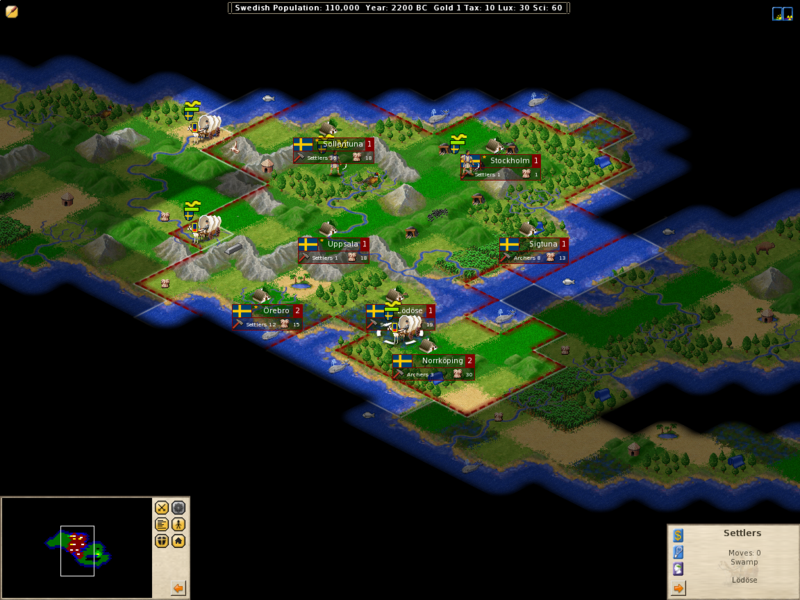
\includegraphics[width=0.65\textwidth,keepaspectratio]{Figures/Chapter1/minimap.png}
% 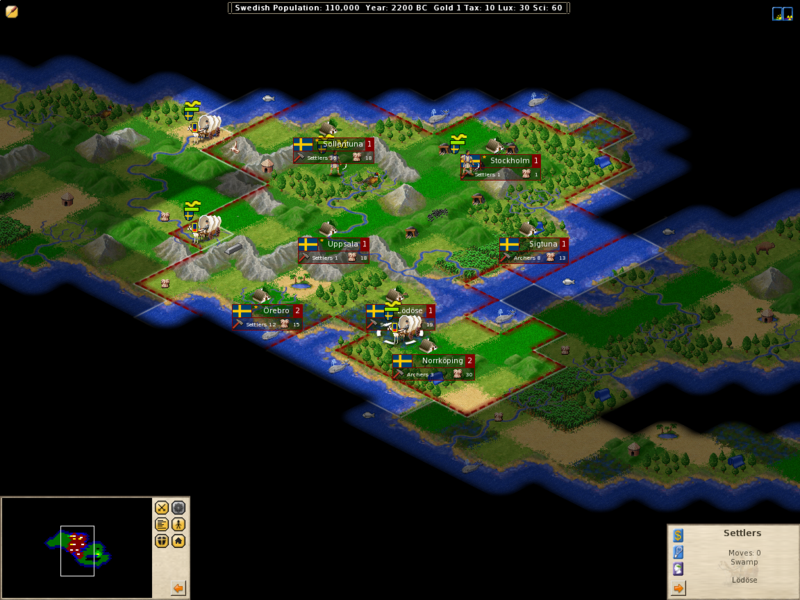
\includegraphics{Figures/Chapter1/minimap.png}
\decoRule
\caption[Overview Plus Detail in Computer Games]{The computer game \emph{Freeciv} has a mini-map in the bottom left corner. This is a similar concept as \gls{opd}. On this mini-map the white rectangle represents the area of the map currently visible on the main screen. The different colors represent land and ocean and the territories of the different players. The white dots are the position of cities and the blackness are the unexplored areas (the ``fog of war'')\cite{wiki:minimap}.}
\label{fig:minimap}
\end{figure}

Note that the term of \emph{Overview + Detail} sometimes are also referred to as \emph{Focus + Context}, \emph{Mini-map} or some other terms, however, they are referring to similar techniques or concepts. 

%----------------------------------------------------------------------------------------
%	SECTION
%----------------------------------------------------------------------------------------

\section{Motivation: Easy Usable Interfaces for Extreme Resolution Datasets}

Most of these techniques and examples above are feasible and can improve how human comprehend the information or datasets, because the whole context area, although larger than the amount of content that one screen can hold, comparing to the focus area, is still not so much bigger. If you're looking at a street plan of a city, the focus area can still be visibly represented as a rectangle if the context area is only as large as a city. If you're looking at an image with the resolution of twice as wide and tall as your screen monitor, the focus area still has a quarter of the size of the context area.

However, there are situations when these techniques will not be able to improve our comprehension of the whole dataset in a very good way, that is when the resolution of the original dataset is getting too high and the focus area is zoomed in into an extremely detailed state. That way, the focus region becomes a ``dot'' instead of a region to be represented on the context view, losing its width and height properties and stops giving intuitive information. A simple example is shown in \gmref{fig:becomespoint} indicating that when the resolution of the dataset is extreme, new approaches need to be taken in order to let the users able to ``grab the whole picture''.

\begin{figure}[H]
\centering
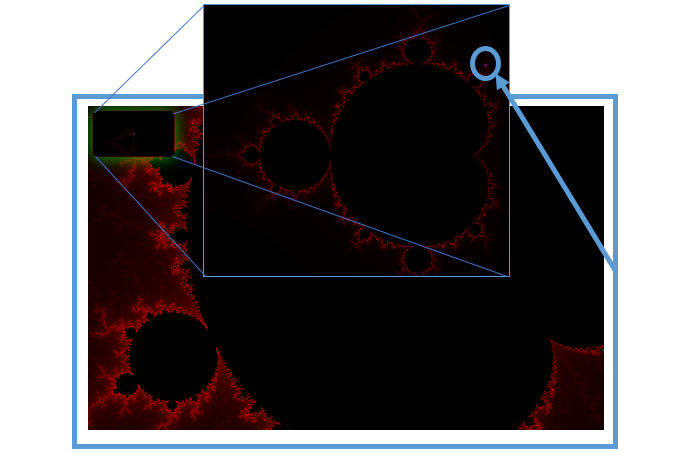
\includegraphics[width=0.85\textwidth,keepaspectratio]{Figures/Chapter1/becomespoint.png}
% 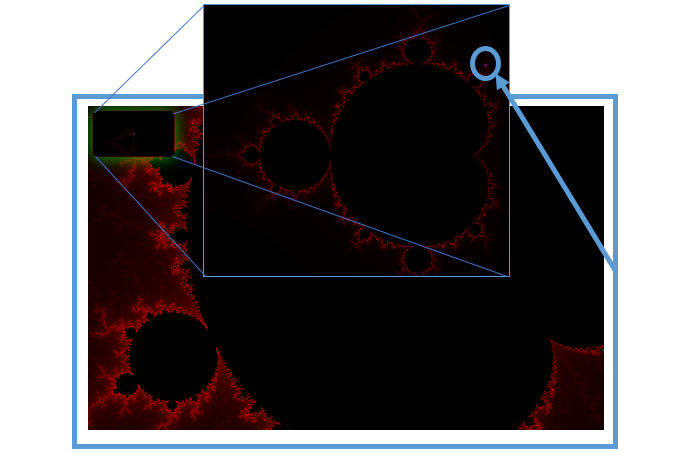
\includegraphics{Figures/Chapter1/becomespoint.png}
\decoRule
\caption[Focus Region Becomes a Dot on Context Region]{Traditional \gls{opd} techniques cannot provide intuitive information on a highly zoomed-in fractal image. For a fractal image this example shows in the overview a point that is in detail a complex pattern.}
\label{fig:becomespoint}
\end{figure}

In these situations, a new level of the \gls{opd} techniques is introduced, which is to provide more levels of overviews to the user. Take what is shown in \gmref{fig:zeus} as an example, multiple levels of information of objects are presented as overviews for the users to browse and search. Instead of an one level solution as shown in \gmref{fig:becomespoint}, the solution shown in \gmref{fig:multiplelevels} gives multiple hierarchical overviews to the user to preserve the intuitiveness of the techniques.

\begin{figure}[H]
\centering
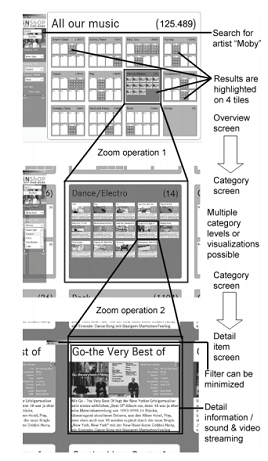
\includegraphics[width=0.35\textwidth,keepaspectratio]{Figures/Chapter1/zeus.png}
% 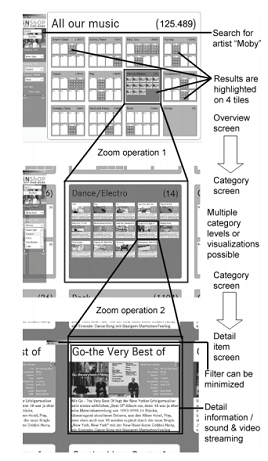
\includegraphics{Figures/Chapter1/zeus.png}
\decoRule
\caption[Multiple Levels of Overview Plus Detail]{ZEUS is an interface that allows hierarchical searching from overview to detail by explorative zooming\cite{gundelsweiler2007zeus}.}
\label{fig:zeus}
\end{figure}

\begin{figure}[H]
\centering
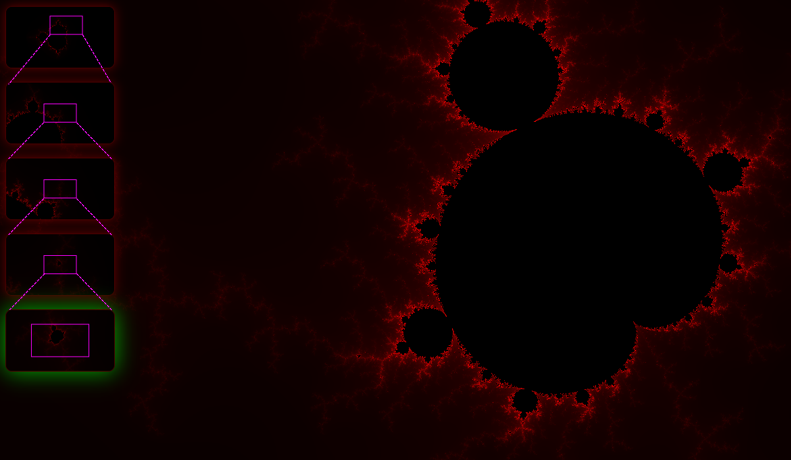
\includegraphics[width=0.9\textwidth,keepaspectratio]{Figures/Chapter1/multiplelevels.png}
% 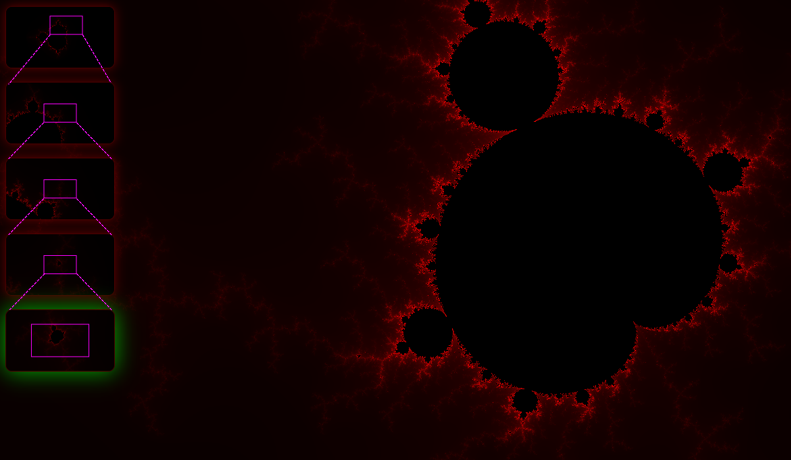
\includegraphics{Figures/Chapter1/multiplelevels.png}
\decoRule
\caption[Zoomed-in Fractal Image]{A graphical representation of Mandelbrot set zoomed in for around $35$ thousand times compared to the original.}
\label{fig:multiplelevels}
\end{figure}

This solution is straightforward, however, we can still raise questions to push the topic into new levels --- what happens when the resolution of the dataset increases even more?

In this case, more overviews need to be added and presented to the users. When more overviews are added providing more \glspl{lod} and contexts and put to the screen, the original problem emerges again --- these overviews are going to occupy a large portion or even the entire screen monitor so the most zoomed-in detail area, the most important area of interest, is not going to be easily comprehended or even not able to be seen, as shown in \gmref{fig:occupiesscreen}. 

\begin{figure}[H]
\centering
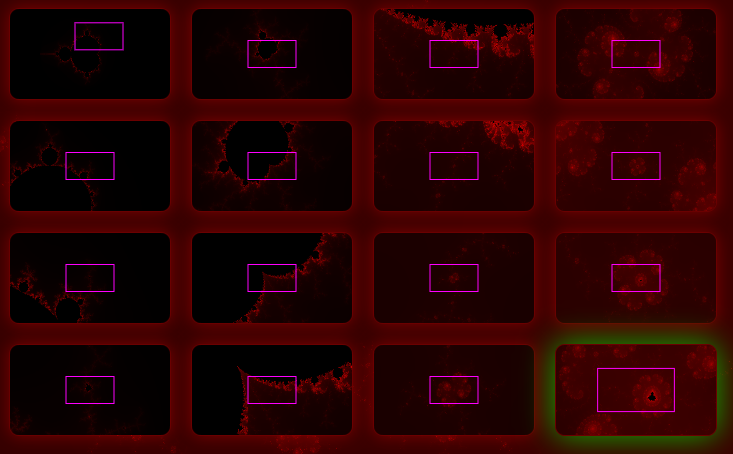
\includegraphics[width=\textwidth,keepaspectratio]{Figures/Chapter1/occupiesscreen.png}
% 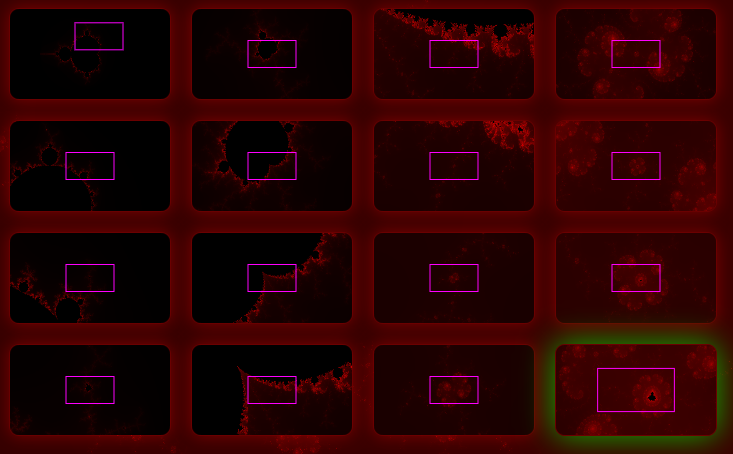
\includegraphics{Figures/Chapter1/occupiesscreen.png}
\decoRule
\caption[Occupied Screen]{Too many overviews occupying entire screen monitor.}
\label{fig:occupiesscreen}
\end{figure}

Therefore, the topic of this thesis is focused on solving this problem, to arrange these overviews in certain ways that they can all provide hierarchies of overviews of information with respect to the original extreme resolution dataset, at the same time, being intuitive enough for human users to understand the \glspl{lod} as well as the most detailed region with the help of all these arrangements.

\section{Inspirations for the Advanced Context Views}

\glsunset{it}

As we mentioned above, in order to prevent situations like shown in \gmref{fig:occupiesscreen} that all tiled context views occupying the entire focus view from happening, we figured out several ways of arranging these context views, and the inspirations of which came from various ways of how we interact with \gls{it} related objects.

\subsection{Dock And Scrollbar}

First thing that came into my mind was the state-of-the-art designs from \emph{Apple}. They invented the concept of macOS Dock or \emph{Dock} as shown in \gmref{fig:macosdock1}, which can be used as an idea of arranging multiple objects of interest on one screen. Not that as shown in \gmref{fig:macosdock1-1}, that it adds an eye-catching visual effect to the current focused object and some other coherent objects.

\begin{figure}[th]
\centering

\includegraphics[width=\textwidth,keepaspectratio]{Figures/Chapter1/macosdock1.png}
% 
\includegraphics{Figures/Chapter1/macosdock1.png}
\decoRule
\caption[MacOS Dock]{Apple gives users the ability to put interested Apps on one side of the screen, which can be the interested contexts in our project.}
\label{fig:macosdock1}
\end{figure}

\begin{figure}[th]
\centering
% 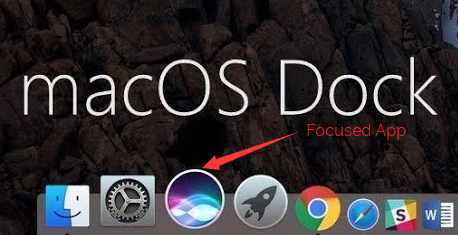
\includegraphics[width=\textwidth,keepaspectratio]{Figures/Chapter1/macosdock1-1.png}
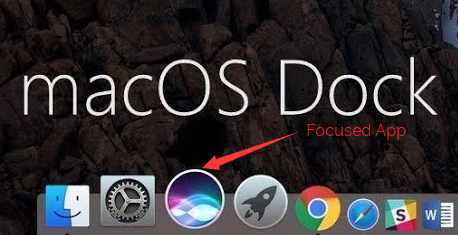
\includegraphics{Figures/Chapter1/macosdock1-1.png}
\decoRule
\caption[MacOS Dock Hover]{When user hovers over an object of interest on the Dock, the Dock can show a visually distinguishable effect.}
\label{fig:macosdock1-1}
\end{figure}

However, in situations that when user tries to add more interested objects to the Dock, this design only shrinks the sizes of the objects and cannot provide capabilities to embody more objects and advance further, as shown in \gmref{fig:macosdock2}.

\begin{figure}[th]
\centering

\includegraphics[width=\textwidth,keepaspectratio]{Figures/Chapter1/macosdock2.png}
% 
\includegraphics{Figures/Chapter1/macosdock2.png}
\decoRule
\caption[MacOS Dock with More Apps]{Apple Dock has certain limitations of holding more objects inside.}
\label{fig:macosdock2}
\end{figure}

To display more object in a smaller container, the obvious way is to put a scrollbar beside, as shown in \gmref{fig:scrollbar}. So the first idea for a new overview technique was born: combining a scrollbar together with the visual effects of the macOS Dock.

\begin{figure}[H]
\centering
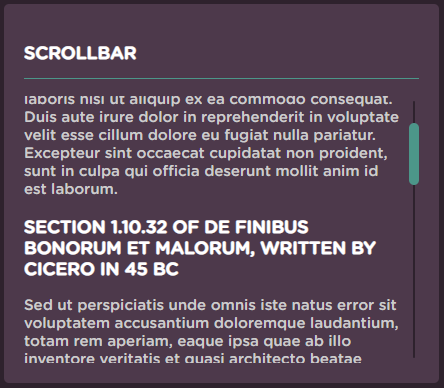
\includegraphics[width=.5\textwidth,keepaspectratio]{Figures/Chapter1/scrollbar.png}
% 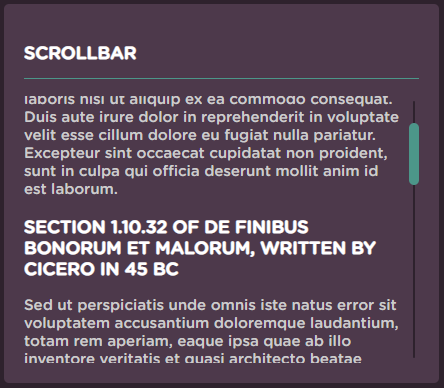
\includegraphics{Figures/Chapter1/scrollbar.png}
\decoRule
\caption[Modern-looking Scrollbar]{An example of using a scrollbar on the side of a container to allow users to browse through more information inside this container.}
\label{fig:scrollbar}
\end{figure}

\subsection{Stacked Cards}

We all browse through different web pages for some information nowadays, and we all had the necessity to keep several web pages open at the same time at some point. The amount of opened websites can easily grow out of hand and how the modern web browsers are handling these web pages of interest can easily catch our attention. The next thing that caught my attention is the \emph{iOS Safari} browser. It is a famous browser installed by default on a popular mobile phone which is a device that has limited amount of space for visual area. How it's displaying the opened web pages are shown in \gmref{fig:iossafari}.

Visually, they look like cards stacked upon each other. What if we arrange it in a way that this stack of cards can dynamically adjust their positions on screen and the angles they pile up with as their numbers grow? This is the next promising idea for arranging context views: stacked cards.

\begin{figure}[th]
\centering
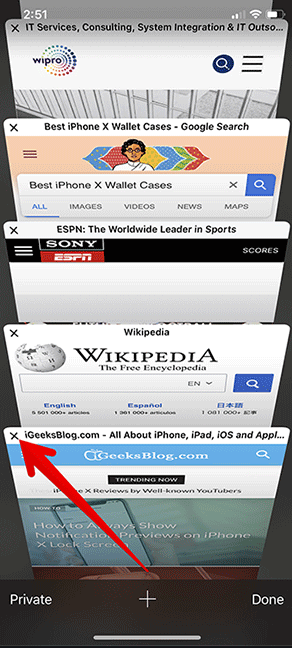
\includegraphics[width=.4\textwidth,keepaspectratio]{Figures/Chapter1/iossafari.png}
% 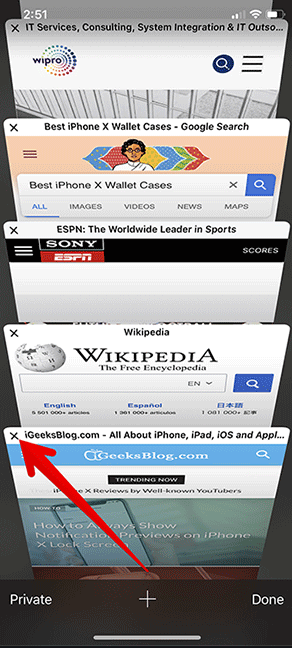
\includegraphics{Figures/Chapter1/iossafari.png}
\decoRule
\caption[Means of Arrangements on iOS Safari]{How iOS Safari arranges multiple open web pages on an iPhone.}
\label{fig:iossafari}
\end{figure}

\subsection{Tabs}

As mentioned before, how browsers arrange the open web pages can be really good examples for our project, therefore, we can't neglect the conventional way of arranging the open web pages on the top of the visual area as ``opened tabs'', like shown in \gmref{fig:tabs}. So we have a third new idea for arranging context views: tabs.

\begin{figure}[H]
\centering

\includegraphics[width=\textwidth,keepaspectratio]{Figures/Chapter1/tabs.png}
% 
\includegraphics{Figures/Chapter1/tabs.png}
\decoRule
\caption[How Google Chrome Arranged Objects of Interest]{The way Google Chrome handles the open web pages are to put a so-called ``tab'' on top of visual area shaped like a tag, with informative titles which sometimes are shortened with ellipsis at the end.}
\label{fig:tabs}
\end{figure}

\subsection{Previews Of Contexts}

\glsunset{pc}

As shown in \gmref{fig:multiplelevels}, the context views can be relatively small when put to action. Therefore, we need some sort of mechanism to let the user ``preview'' the shrunk context views, in a similar sense where \emph{Windows 10} users can hover their cursor over the bottom right corner of their screen to have a ``glance'' of how their desktop looks like shown in \gmref{fig:winpreview}, hiding the \gls{ui} of the current open applications.

\begin{figure}[H]
\centering
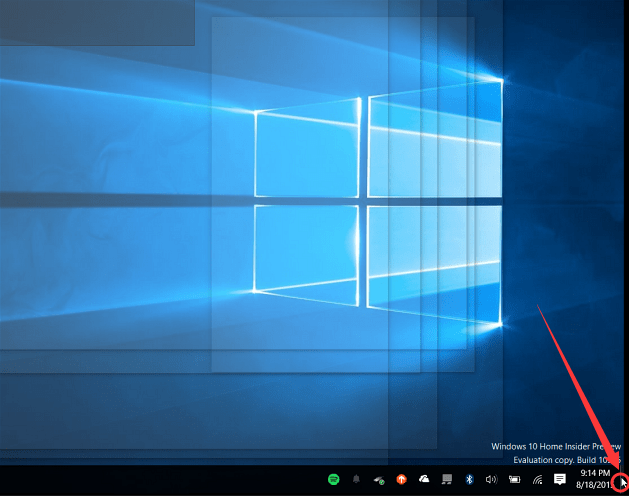
\includegraphics[width=\textwidth,keepaspectratio]{Figures/Chapter1/winpreview.png}
% 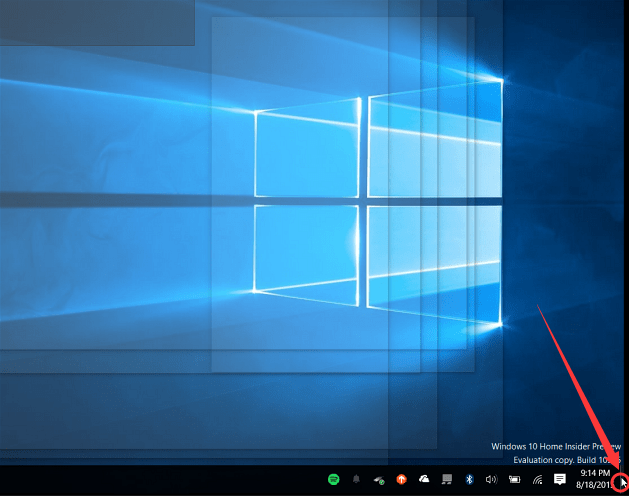
\includegraphics{Figures/Chapter1/winpreview.png}
\decoRule
\caption[``Preview'' Mechanism on Windows 10]{When users hover their mouse cursor on bottom right corner of a Windows \gls{pc} and have a glance of what is on their Desktop.}
\label{fig:winpreview}
\end{figure}

A most natural preview setup would be like this, when the user hovers over one of the context view, display an enlarged image in \gls{fhd} that shows the context. That is in fact the default setting of this project.

As inspired by the same \emph{Windows} effect, the second visual effects type becomes a fade-in and fade-out effect. This effect, as shown in \gmref{fig:jqfadein}, is adding a small transition in the transparencies of the context to be displayed on screen --- smoother and can give positive user experience in the comprehension of the \gls{fpc} problem.

\begin{figure}[H]
\centering
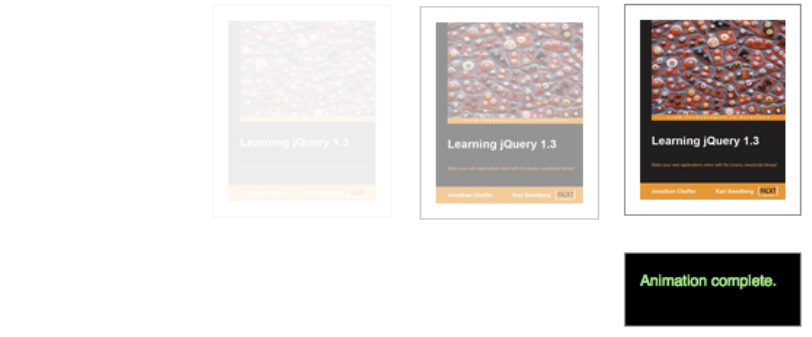
\includegraphics[width=\textwidth,keepaspectratio]{Figures/Chapter1/jqfadein.png}
% 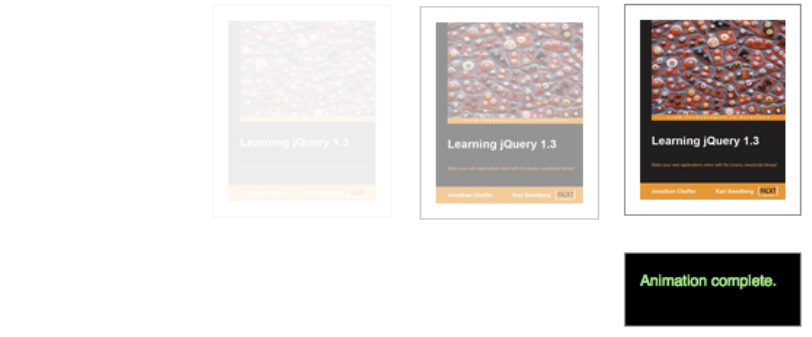
\includegraphics{Figures/Chapter1/jqfadein.png}
\decoRule
\caption[Fade-in Effect in jQuery]{Illustration of the \texttt{fadeIn()} effect in \emph{jQuery}, a transparency change of objects to be displayed.}
\label{fig:jqfadein}
\end{figure}

Another way of giving previews of the contexts is inspired by some modern graphics and video work, such as a deep zooming video of Mandelbrot set\footnote{ See \url{https://www.youtube.com/watch?v=pCpLWbHVNhk} for more information.} or some special scenes in a movie such as ``Limitless''\footnote{ See \url{https://www.youtube.com/watch?v=xqv1maJaDtQ&t=37} for more information} or ``Man In Black''\footnote{ See \url{https://www.youtube.com/watch?v=OKnpPCQyUec} for more information.}.

As shown in \gmref{fig:zoompreview}, it would be really nice if we implement this visual feature that when user wants to preview one of the contexts, instead of magically showing that context, we show this process of letting the preview image raise or sink from the ``current'' depths to the ``intended'' depths of the context. Therefore, this second ways of previewing the contexts got to be implemented into this project.

\begin{figure}[H]
\centering
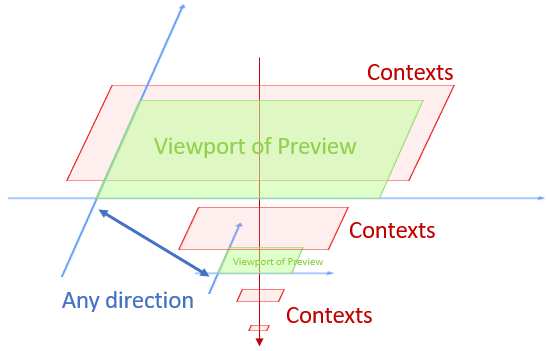
\includegraphics[width=.8\textwidth,keepaspectratio]{Figures/Chapter1/zoompreview.png}
% 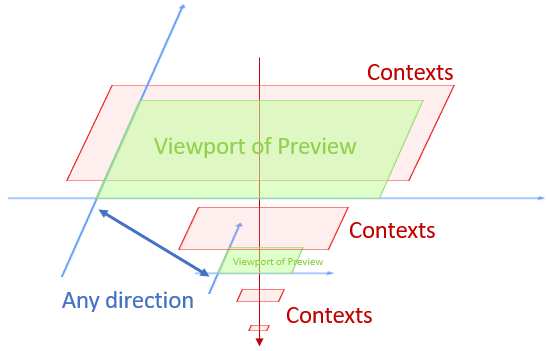
\includegraphics{Figures/Chapter1/zoompreview.png}
\decoRule
\caption[Moving Preview Plane on Context Views]{The viewport of preview is like a plane raising or sinking to the desired depths on the \texttt{z} axis.}
\label{fig:zoompreview}
\end{figure}

%----------------------------------------------------------------------------------------
%	SECTION
%----------------------------------------------------------------------------------------

\section{Related Work}

There are many researchers who have already done plenty of work related to the topic of \gls{opd}, \gls{fpc} or \gls{lod}.

Some researchers did work on a single level of \gls{fpc} techniques:

Cockburn et al. \cite{cockburn2006review, cockburn2009review} reviewed and compared \gls{opd}, zooming, and \gls{fpc} interfaces. They described that \gls{opd} uses a spatial separation between focused and contextual views, zooming is temporal separation of views and \gls{fpc} displays the focus within the context.

Hornb{\ae}k et al. \cite{hornbaek2002navigation} compared zoomable user interfaces with and without an overview by experiments to understand the navigation patterns and usability of these interfaces. In a later work, Hornb{\ae}k et al. \cite{hornbaek2011notion} extensively reviewed papers that used the notion of overview and developed a model which highlights the awareness that makes up an overview, the process, by which users acquire it, the usefulness of overviews, and the role of user-interface components in developing an overview.

Baudisch et al. considered mainly the technique focus plus context screens.\cite{baudisch2002keeping} They experimented and compared this technique with the other two techniques overview plus detail and zooming/panning. They noted, for interaction with dynamic views, the technique focus plus context screens alone seems not to be enough and needs an additional monitor. In a related work, Baudisch et al. \cite{baudisch2001focus} present the technique focus plus context screens and implemented a system with this technique by combining multiple display units of different resolution. Their means is particularly suitable for situations where all information is shown in only one view and switching between multiple views should be avoided.

Roto et al. \cite{roto2006minimap} developed a Web page visualization method minimap for mobile phones that shows pages in a modified original layout and navigates a Web page with a mini map view. A red rectangle in minimap corresponds to the current location in the detail view. The minimap content is transparent. The user may adjust the opacity level through the browser preferences. Furthermore, and most importantly, the overview becomes visible only when the user is scrolling the document.

Gutwin et al. \cite{gutwin2004interacting} compared three techniques: fisheye, zoom and panning, to find out what is the best ways to redesign a large UI to fit a smaller screen of mobile devices.

Holmquist \cite{holmquist1998zoom} developed a flip zooming as a new focus+context technique: Mini Pages are placed in a simple left-to-right, top-to-bottom ordering on the display. When a page is brought into focus, it is enlarged and placed approximately in the middle of the display, with the other Mini Pages arranged around it.

There are also some researchers did work related with multiple \glspl{lod}:

Pan et al. \cite{zhigeng1998overview} present a summary on the mesh simplification techniques which they used for creating models at multiple \gls{lod}. In this paper they also compared typical methods.

Clark \cite{clark1976hierarchical} proposed hierarchical geometric models for visible surface algorithms for producing computer pictures. He described the benefits of using more than one representation of a model for image rendering and pointed out that objects that cover a small area of the screen can be rendered from a simplified version of the object and that this allows more efficient rendering of a scene.

Crow \cite{crow1982more} described the benefits of having both simple and complex representations of an object in his paper on an image generation environment. He gave an example of a chair that is represented in high detail, medium detail and very low detail. These models with three level of detail were created by hand. He suggested that creating the lower levels of detail is a process that should be automated.

Gundelsweiler et al. \cite{gundelsweiler2007zeus} developed a system of hierarchical information structure. Objects and categories are organized in groups on different hierarchy level visualized as tiles on the screen by the user. The search is supported by zooming/panning navigation.


% ---

% Single level:

% 1. A Review of Overview+Detail, Zooming, and Focus+Context Interfaces\cite{cockburn2009review}

% 2. A Review of Focus and Context Interfaces\cite{cockburn2006review}

% 3. Navigation Patterns and Usability of Zoomable User Interfaces with and without an Overview\cite{hornbaek2002navigation}

% 4. Keeping Things in Context: A Comparative Evaluation of Focus Plus Context Screens, Overviews, and Zooming\cite{baudisch2002keeping}

% 5. Focus Plus Context Screens: Combining Display Technology with Visualization Techniques\cite{baudisch2001focus}

% 6. Minimap – A Web Page Visualization Method for Mobile Phones\cite{roto2006minimap}

% 7. Interacting with Big Interfaces on Small Screens: a Comparison of Fisheye, Zoom, and Panning Techniques\cite{gutwin2004interacting}

% 8. The notion of overview in information visualization\cite{hornbaek2011notion}

% 9. The Zoom Browser: Showing Simultaneous Detail and Overview in Large Documents\cite{holmquist1998zoom}


% Multiple level:

% 10. Overview of Multiple Level of Detail Creation\cite{zhigeng1998overview}

% 11. Hierarchical geometric models for visible surface algorithms\cite{clark1976hierarchical}

% 12. A more flexible image generation environment\cite{crow1982more}

% 13. ZEUS–zoomable explorative user interface for searching and object presentation\cite{gundelsweiler2007zeus}
% Chapter Template

\chapter{Background} % Main chapter title

\label{Chapter2} % Change X to a consecutive number; for referencing this chapter elsewhere, use \ref{ChapterX}

In this chapter, we will introduce some necessary background knowledge in order to let the reader understand better how this project came into its form.

Not only the technology stack that this project used is important to further understanding, but also some theoretical part that's behind. We shall introduce it gradually.

%----------------------------------------------------------------------------------------
%	SECTION
%----------------------------------------------------------------------------------------

\section{Web Technology Stack}

Before starting to program on the software that shows the different ways to show an interface providing \gls{fpc} with many \gls{lod}, we must first choose the nature and language of the program. A web technology stack program stands out easily and as a matter of fact, was also the first choice for the development of the immature prototype in the first place. There are several reasons behind it. For web technology stack developed programs:

\begin{itemize}
    \item \textbf{Compatibility} Code once, it works everywhere. It saves lots of time for users and testers to read a long manual. All we need is a working browser with loose requirements to it.
    \item \textbf{Simple Installation} Almost nothing to be installed in order to see the project up and running. Besides a browser of some version specifications, only a web server of \emph{any kind} is required, as described in \gmref{chap4:starttheproject}.
    \item \textbf{Appearance} Can look modern with almost zero code. Can have cool visual effects a lot easier than desktop development. 
    \item \textbf{Successful Case} If it works for Google Maps, it should work for our project as well.
    \item \textbf{Performance} Slower in a sense because hardware resources are not easily fetched for browser-based \gls{ui} heavy applications.
\end{itemize}

On the other hand for desktop development:

\begin{itemize}
    \item \textbf{Compatibility} Really common to be ``working on my computer'' but not on users'.
    \item \textbf{Simple Installation} Lots of preconditions and require lots of planning before the delivery of a standalone package. If not planned and all aspects chosen carefully, applications might not work on Macs and gives pop-ups to require ``vcredist'' dependencies on other operating systems.
    \item \textbf{Appearance} Requires lots of coding to have the most basic appearance. Visual effects need to be programmed manually one by one, not to mention the planning of the software structure. 
    \item \textbf{Successful Case} Works also fine with lots of deep zooming applications such as \emph{Ultra Fractal} and \emph{Kalles Fraktaler}.
    \item \textbf{Performance} Can be a lot faster than web applications if choosing \emph{C} / \emph{C++} or similar languages since they can access directly your hardware resources.
\end{itemize}

Since this project is focused a lot on the front end \gls{ui}, web technologies is chosen even when performance can sometimes hinder the advancement of some applications. If planned well, performance on the deep zooming part of the project can be improved by coding techniques and algorithms, however, on the other hand, programming front end \gls{ui} effects together with planning a good structure to use the advantages of calculation speed of desktop applications would not be productivity efficient.

\glsunset{gpu}
\glsunset{cpu}

Some other approaches were also considered, for example to use an intermediate solution like Python because it can be easily structured and coded, however, most of them were not as good choices as web technologies. Taking Python as an example, it cannot do conventional iterations over pixels fast enough unless complicated techniques are used, which actually brings it back on the same level with desktop programming, not to mention the invocation of hardware \gls{gpu} / \gls{cpu} resources and fast image manipulations --- they all bring lots of complications to the implementation of the project.

%----------------------------------------------------------------------------------------
%	SECTION
%----------------------------------------------------------------------------------------

\section{Web, HTML5 And Canvas API}

After the choice of web technology stack, we'll be talking about the equipments that are used in the project.

Technically speaking, web wechnologies are focused on \gls{ui} and communications between servers and computers since the computers and servers on the internet can't communicate with each other the way people do, however, the communication part is not hugely focused in this project. First thing to know is that web technology stack includes the markup languages and multimedia packages servers and computers use to communicate, however, it's the markup languages and multimedia packages that we focus on, not the communication part, since the communication involved currently is still on local machines.

\subsection{Browsers}

Web technology runs on browsers. Browsers are the tools that request information and then they show us users in the way we can understand, as the interpreters of the web programs. There are many famous web browsers around:

\begin{itemize}
    \item \textbf{Google Chrome} Currently the most popular browser by Google
    \item \textbf{Safari} Apple's web browser
    \item \textbf{Firefox} Open-source browser supported by the Mozilla Foundation
    \item \textbf{Internet Explorer} Microsoft's browser
\end{itemize}

And since Google Chrome has the most popularity and supports all of our requirements for the project, we chose Google Chrome as our browser for the project.

\subsection{Markup Language}

There are some fundamental things for web programming. The first things we need to know about are \gls{html}, \gls{css} and \gls{js}.

\paragraph{HTML}

\gls{html} is one of the first thing to be introduced in this section. Thanks to \gls{html}, the browsers can know what to present when we hit them we a request. It is the standard markup language for documents designed to be displayed in a web browser. It can be assisted by technologies such as \gls{css} and scripting languages such as \gls{js}.\cite{wiki:html}

\paragraph{CSS}

\glsreset{js}

The technology assisting \gls{html} describes how \gls{html} elements are to be displayed on the screen, if to be put straightforward. It is a style sheet language used for describing the presentation of a document written in a markup language like \gls{html}.\cite{wiki:css} \gls{css} is a cornerstone technology of the web technologies, alongside \gls{html} and \gls{js}.\cite{flanagan2006javascript}

\paragraph{JavaScript}

\glsreset{js}

Alongside \gls{html} and \gls{css}, \gls{js} is one of the core technologies of the World Wide Web.\cite{flanagan2006javascript} JavaScript enables interactive web pages and is an essential part of web applications. The vast majority of websites use it,\cite{w3techs2018usage} and major web browsers have a dedicated JavaScript engine to execute it.\cite{wiki:js}

\subsection{HTML5}\label{chap2:html5}

It is worth mentioning that there is more to the technologies this project is using than the traditional \gls{html} / \gls{css} / \gls{js}, which is the larger set --- \gls{h5}. \gls{h5} is the latest evolution of the standard that defines the original. The term \gls{h5} represents two different concepts:

\begin{itemize}
    \item It is a new version of the markup language \gls{html}, with new elements, attributes, and behaviors
    \item A larger set of new web technologies that allows the building of more diverse and powerful applications.
\end{itemize}

Therefore, this set is sometimes called \emph{\gls{h5} and friends} and often shortened to just \gls{h5}.

There are lots of new features that \gls{h5} brings to the original \gls{html}, but we're not describing all them there in full\footnote{ See \url{https://en.wikipedia.org/wiki/HTML5} to know more details}. The core features we care about and using in this project are the following two:

\paragraph{Graphics and Effects} Allowing a much more diverse range of presentation options, with respect to 2D / 3D graphics and effects.
\paragraph{Performance and Integration} Providing greater speed optimization and better usage of computer hardware.
\paragraph{Styling} Allowing more sophisticated themes and \gls{ui} experience.

Solving exactly the problems of our focus points in this thesis. Some more specific details to each of the above points and their applications in this project will be shortly described.

In the graphics part, the new element \texttt{<canvas>} element that allows delicate drawing on web pages are heavily used. 

In the performance and integration part, \emph{Web Worker}s are used allowing delegation of \gls{js} evaluation to background threads, preventing these operations from slowing down \gls{ui} interactive events. The separation used in the project can also be easily advanced by replacing this multithreading calculation part with the new \emph{XMLHttpRequest} allowing fetching information asynchronously, also allowing it to display dynamic content, varying according to the time and user actions\footnote{ This is the technology behind \emph{Ajax}. To know more information about \emph{Ajax}, see \url{https://en.wikipedia.org/wiki/Ajax_(programming)}.}. 

In the styling part, since the new \gls{css} in \gls{h5}, \gls{css3}, has been extended to be able to style elements in a much more complex way, many new features of \gls{css3} are used, such as:

\paragraph{Background Styling}

The possibility to put shadows on elements using \texttt{box-shadow} and \gls{css} \texttt{filter}s. These advanced box effects are used in this project for the display of halos of the context views and also internally in the dependencies of this project, \emph{jQuery}\footnote{ jQuery is an open-source, fast, small, and feature-rich JavaScript library. It makes things like HTML document traversal and manipulation, event handling, animation, and Ajax much simpler with an easy-to-use API that works across a multitude of browsers. See \url{https://jquery.com/} for more information.} and \emph{Bootstrap}\footnote{ Bootstrap is an open source toolkit for developing with \gls{html}, \gls{css}, and \gls{js}. See \url{https://getbootstrap.com/} for more information.}.

\paragraph{Animating of Styles}

Using CSS Transitions to allow the animation between different states or using \emph{\gls{css} Animations} to animate parts of the page without a triggering event, for example some movement animations of the context views in this project.

\paragraph{New Presentational Layouts}

Two new layouts have been added to \gls{css3}: the \gls{css} multi-column layouts and \gls{css} flexible box layout, and the latter is used in multiple places in this project, for example, the default layouts for the context views and the tabs layouts for the conext views. The dependency \emph{Bootstrap} also relies largely on this new feature.

\subsection{Canvas API}

\gls{h5} brought exciting new advantages to the \gls{html} coding world as mentioned above. Amongst them all, one of the most thrilling one, the new \texttt{<canvas>}, allows us to render delicate graphics powered by \gls{js}. We'll be talking about what it is and then the \gls{api} that supports its usages.

\texttt{<canvas>} is an \gls{html} element which can be used to render graphics via scripts\footnote{ To know about the \texttt{<canvas>} element, see \url{https://en.wikipedia.org/wiki/Canvas_element}.}, here in our project \gls{js}. It can, for instance, be used to draw graphs or create simple (and not so simple) animations. In our project, \texttt{<canvas>} is used for the graphical representation of the extreme resolution datasets.

It's also worth mentioning that after first introduced in \emph{WebKit} by \emph{Apple} for the \emph{OS X Dashboard}, \texttt{<canvas>} has since been implemented and supported in all major browsers today.

The Canvas \gls{api} itself is a sense of how to use scripts to draw on this newly introduced \gls{html} element. It is largely focuses on 2D graphics. The reason to bring it up here together with the \texttt{<canvas>} element is that there are many other \gls{api}s that come together with it, for example the WebGL \gls{api}, which also uses the \texttt{<canvas>} element, draws hardware-accelerated 2D and 3D graphics. In another word, the context of the \texttt{<canvas>} element\footnote{ Here not the same concept as the ``context'' in the previously mentioned term \gls{fpc}.} is ``2d'' through the Canvas \gls{api}, not ``webgl'' context or any other.

%----------------------------------------------------------------------------------------
%	SECTION
%----------------------------------------------------------------------------------------

\section{Mandelbrot Set}

As for the datasets themselves, we use a kind of computable dataset instead of a static and deep zoomable image information dataset. The advantage is obvious that by using a dataset that can be computed for its information of any specific point in the set, we don't have to store the information anywhere anymore, as if we did, it would require a lot of investment and investigation for the storage or fetching of the dataset for this project. The downside of it is also clear that we'll have to trade time for space, since the calculation is usually going to take more time than only querying from a static set of data. It is proved to be solid to do this trade, since in this project, the visually inspected results shows that the waiting time is still inside human tolerable margins.

The dataset we chose is the Mandelbrot set. The Mandelbrot set is a famous example of a fractal in mathematics. It is named after Beno\^{\i}t Mandelbrot, a Polish-French-American mathematician\footnote{ Its definition and name are due to Adrien Douady, in tribute to the mathematician Beno\^{\i}t Mandelbrot\cite{wiki:mandel}.}. The reason this thesis is using Mandelbrot set as the source of extreme resolution dataset is because Mandelbrot set can provide theoretically infinitely high resolution datasets. In this section, we'll introduce briefly Mandelbrot set, its algorithms ideas for visualization.

\subsection*{What Is Mandelbrot Set}

Firstly, we recursively define a sequence $\displaystyle (z_{n})_{n\in\mathbb{N}},\thickspace z_{n}\in\mathbb{C}$ as follows:

\begin{equation}
    z_0 = 0
\end{equation}

\begin{equation}
    z_{n} = z_{n-1}^2 + c,\thickspace c\in\mathbb{C}
\end{equation}

For different constant $c$, the absolute value of $z_n$ could remain bounded, could also be divergent, if $n$ is increased.

The Mandelbrot set $\mathbb{M}$ is the set of $c$ in the complex plane for which the sequence $\displaystyle (z_{n})_{n\in\mathbb{N}},\thickspace z_{n}\in\mathbb{C}$ remains bounded.

\subsection*{Important Properties of the Mandelbrot Set}

A property of Mandelbrot set is as follows:

A complex number $c$ belongs to the Mandelbrot set $\mathbb{M}$, if and only if the absolute value of $z_n$ is not larger than $2$, for all $n = 0, 1, 2, ..$

\subsection*{Simple Graphical Presentation}

The following figure \gmref{fig:mandelbrot} is a simple graphical representation of Mandelbrot set. A point $c$ in the complex plane is conventionally colored \emph{black} if it belongs to the Mandelbrot set $\mathbb{M}$, and \emph{white} if not. 

\begin{figure}[th]
\centering
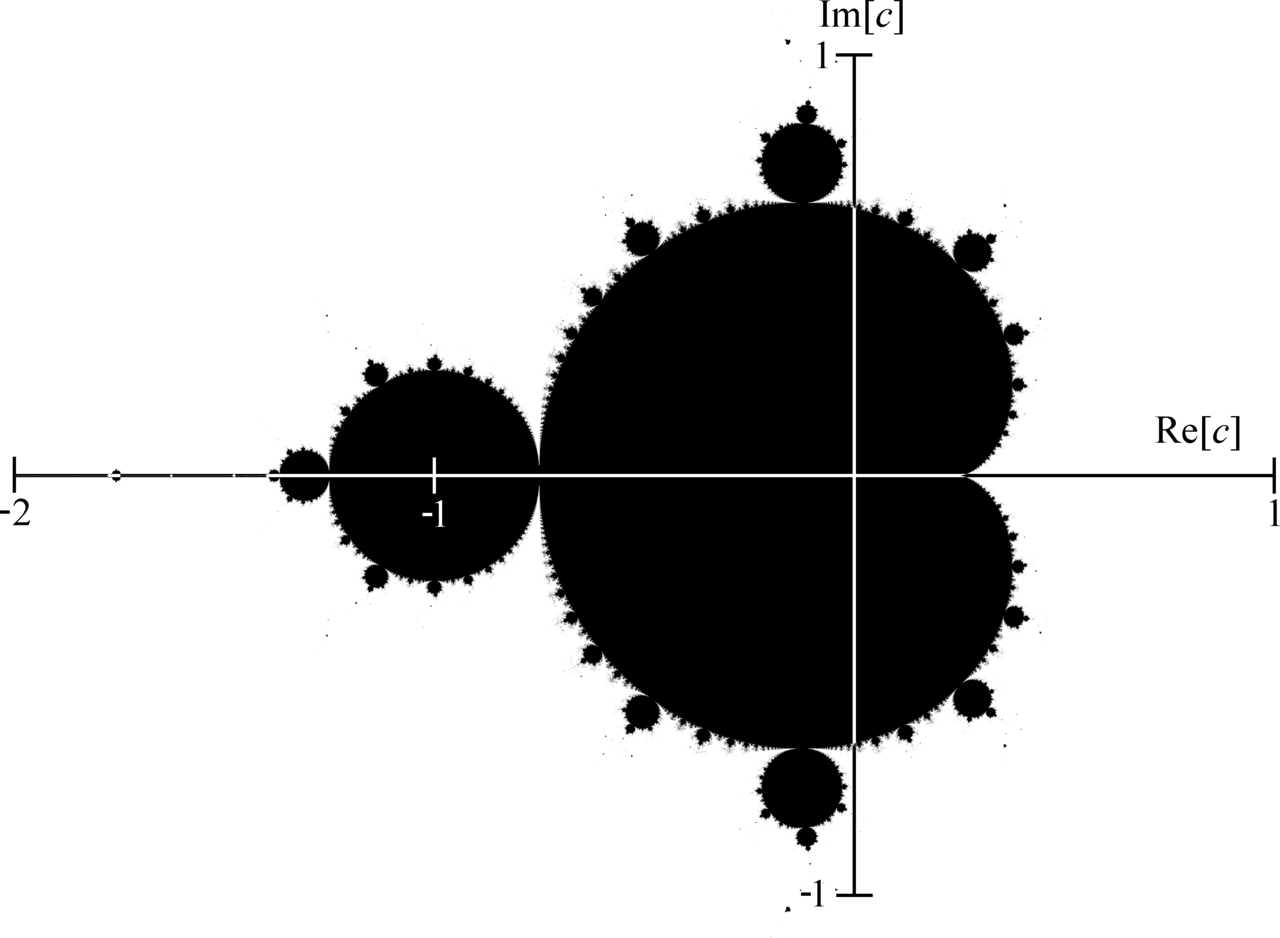
\includegraphics[width=\textwidth,keepaspectratio]{Figures/Chapter2/mandelbrot.png}
% 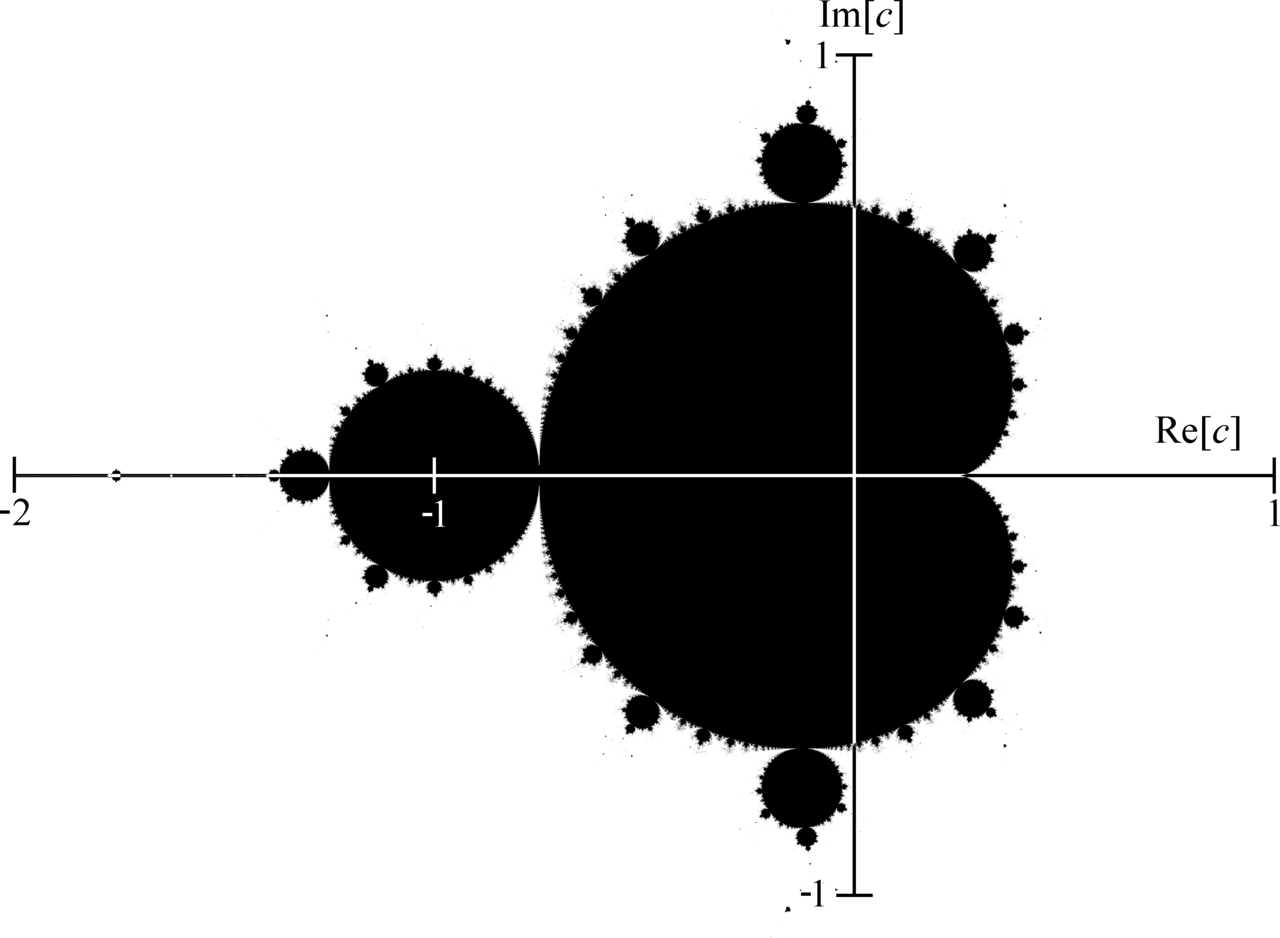
\includegraphics{Figures/Chapter2/mandelbrot.png}
\decoRule
\caption[Mandelbrot Set Graphical Presentation]{A simple graphical representation of Mandelbrot set.}
\label{fig:mandelbrot}
\end{figure}

\subsection*{Algorithms for Visualization}\label{chap2:algorithmsforvisualization}

A simple algorithm is introduced for visualization of black and white in \gmref{alg:simple}.

\begin{algorithm}[H]
    \ForEach{$c$ in complex plane}{
        $z_0 = 0$\;
        \For{$n \leftarrow 0$ \KwTo $max$}{
            $z_n = z_{n - 1}^2 + c$\;
            \If{the value of $z_n$ is larger than $2$}{
                $c$ does not belong to $\mathbb{M}$. In this case, we set the color of $c$ to \emph{white} and the calculation of sequence is stopped\;
            }
            \uElseIf{$n = max$}{
                $c$ belongs to $\mathbb{M}$ and we set the color of $c$ to \emph{black}\;
            }
        }
    }
    \caption{Algorithms for Simple Visualization}
    \label{alg:simple}
\end{algorithm}

In \gmref{alg:simple}, the variable $max$ can be treated as a constant for each complete cycle of the execution of the algorithm. The larger $max$ is, the more accurate the image generated will be. However, it should not be set infinitely large as a point belonging to the Mandelbrot set will cause the algorithm to loop infinitely. A simple equation is used for the determination of this value $max$:

\begin{equation}
    \label{eq:max}
    {(50 \cdot log_{\thinspace 10 \thinspace}{magnif})}^{1.08}
\end{equation}

Where $magnif$ is the magnification level, a number representing the number of pixels that together has a length of $1$ on the mathmatical axis, shown in \gmref{fig:magnif}.

\subsection*{Algorithms Idea for Graphical Representation with Grayscale}

In the mentioned algorithm \gmref{alg:simple}, $c$ is set to either \emph{black} or \emph{white}. If the iteration number $n$ is equal to the maximum iteration number $max$ and the value of $z_n$ still less than $2$, then $c$ has the color \emph{black}. If the iteration number $n$ is smaller than $max$ then at this moment the absolute value of $z_n$ becomes larger than $2$. In this case, we cannot set the color of $c$ to \emph{black}, because $c$ dose not belong to Mandelbrot set. However, we set a color with a portion of \emph{black}, to indicate how close $c$ is to be in \emph{black} area, as shown in \gmref{alg:grayscale}.

\begin{algorithm}[H]
    \ForEach{$c$ in complex plane}{
        $z_0 = 0$\;
        \For{$n \leftarrow 0$ \KwTo $max$}{
            $z_n = z_{n - 1}^2 + c$\;
            \If{the value of $z_n$ is larger than $2$}{
                $c$ does not belong to $\mathbb{M}$\;
                In this case, we set the color of $c$ to \st{\emph{white}} \emph{grayscale\footnote{ In the current implementation, this color is set to be grayscaled red, rgb($grayscale\% \times 255$, 0, 0).} depending on the number of iteration} $n$ and the calculation of sequence is stopped\;
            }
            \uElseIf{$n = max$}{
                $c$ belongs to $\mathbb{M}$ and we set the color of $c$ to \emph{black}\;
            }
        }
    }
    \caption{Algorithms for Grayscale Visualization}
    \label{alg:grayscale}
\end{algorithm}

The value $max$ is determined in the same way as described in \gmref{eq:max}.
% Chapter Template

\chapter{Theoretical Basis} % Main chapter title

\label{Chapter3} % Change X to a consecutive number; for referencing this chapter elsewhere, use \ref{ChapterX}

%----------------------------------------------------------------------------------------
%	SECTION 1
%----------------------------------------------------------------------------------------

\section{Main Section 1}

Lorem ipsum dolor sit amet, consectetur adipiscing elit. Aliquam ultricies lacinia euismod. Nam tempus risus in dolor rhoncus in interdum enim tincidunt. Donec vel nunc neque. In condimentum ullamcorper quam non consequat. Fusce sagittis tempor feugiat. Fusce magna erat, molestie eu convallis ut, tempus sed arcu. Quisque molestie, ante a tincidunt ullamcorper, sapien enim dignissim lacus, in semper nibh erat lobortis purus. Integer dapibus ligula ac risus convallis pellentesque.

%-----------------------------------
%	SUBSECTION 1
%-----------------------------------
\subsection{Subsection 1}

Nunc posuere quam at lectus tristique eu ultrices augue venenatis. Vestibulum ante ipsum primis in faucibus orci luctus et ultrices posuere cubilia Curae; Aliquam erat volutpat. Vivamus sodales tortor eget quam adipiscing in vulputate ante ullamcorper. Sed eros ante, lacinia et sollicitudin et, aliquam sit amet augue. In hac habitasse platea dictumst.

%-----------------------------------
%	SUBSECTION 2
%-----------------------------------

\subsection{Subsection 2}
Morbi rutrum odio eget arcu adipiscing sodales. Aenean et purus a est pulvinar pellentesque. Cras in elit neque, quis varius elit. Phasellus fringilla, nibh eu tempus venenatis, dolor elit posuere quam, quis adipiscing urna leo nec orci. Sed nec nulla auctor odio aliquet consequat. Ut nec nulla in ante ullamcorper aliquam at sed dolor. Phasellus fermentum magna in augue gravida cursus. Cras sed pretium lorem. Pellentesque eget ornare odio. Proin accumsan, massa viverra cursus pharetra, ipsum nisi lobortis velit, a malesuada dolor lorem eu neque.

%----------------------------------------------------------------------------------------
%	SECTION 2
%----------------------------------------------------------------------------------------

\section{Main Section 2}

Sed ullamcorper quam eu nisl interdum at interdum enim egestas. Aliquam placerat justo sed lectus lobortis ut porta nisl porttitor. Vestibulum mi dolor, lacinia molestie gravida at, tempus vitae ligula. Donec eget quam sapien, in viverra eros. Donec pellentesque justo a massa fringilla non vestibulum metus vestibulum. Vestibulum in orci quis felis tempor lacinia. Vivamus ornare ultrices facilisis. Ut hendrerit volutpat vulputate. Morbi condimentum venenatis augue, id porta ipsum vulputate in. Curabitur luctus tempus justo. Vestibulum risus lectus, adipiscing nec condimentum quis, condimentum nec nisl. Aliquam dictum sagittis velit sed iaculis. Morbi tristique augue sit amet nulla pulvinar id facilisis ligula mollis. Nam elit libero, tincidunt ut aliquam at, molestie in quam. Aenean rhoncus vehicula hendrerit.
% Chapter Template

\chapter{Implementation} % Main chapter title

\label{Chapter4} % Change X to a consecutive number; for referencing this chapter elsewhere, use \ref{ChapterX}

In this chapter, the overall structure of the project, how the files are arranged and the functionalities of each components, will be described in details.

%----------------------------------------------------------------------------------------
%	SECTION 
%----------------------------------------------------------------------------------------

\section{Files And Folders}

The folder names and file names are mostly self-explanatory or conventional in this project. They'll be described briefly in this section.

\begin{figure}[th]
\centering
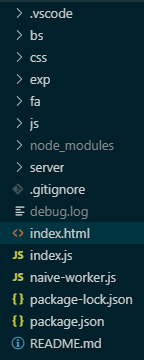
\includegraphics{Figures/Chapter4/filestructure.png}
\decoRule
\caption[File Structure]{A glimpse of files and folders.}
\label{fig:filestructure}
\end{figure}

\subsection{Folders}

\paragraph{Folder \texttt{./.vscode}}

The configured Visual Studio Code workspace settings file. This file is included and stored inside the workspace and only apply when the workspace is opened which overrides Visual Studio Code's default user settings. The author tweaked this file to make some parts of VS Code's editor, user interface, and functional behavior more fitting to review or to base future work upon this project\footnote{ To learn more about this file, see \url{https://code.visualstudio.com/docs/getstarted/settings}.}. 

VS Code provides two different scopes for settings:

\begin{itemize}
  \item User Settings - Settings that apply globally to any instance of VS Code you open.
  \item Workspace Settings - Settings stored inside your workspace and only apply when the workspace is opened.
\end{itemize}

Workspace settings override user settings\cite{bib:ms:vscode}.

\paragraph{Folder \texttt{./js}}

All the third-party open source \gls{js} dependencies are stored in this folder. Sometimes third-party open source projects include a bundle of \acrfull{js} and \gls{css} files, here only the pure \gls{js} projects' files are included.

\paragraph{Folder \texttt{./css}}

The \gls{css} files of the projects are included. Firstly there is a \\\texttt{./css/common.css} file, which sets the overall styles of the project, basically whatever the users can see at the very first glance when they open this project. Then there are several other \gls{css} files, each sets a specific portion of the styles in this project. These files include:

\begin{itemize}
\item \gls{css} File \texttt{./css/dock.css} sets the iOS-Dock look-like styles, making the focused item larger with larger margins and adjacent items smaller and smaller margins with their corresponding nearby items.
\item \gls{css} File \texttt{./css/minibar.css} sets the customed scrollbar styles that's being added upon the default styles of the dependency \emph{MiniBar} which is used to create custom scrollbars.
\item \gls{css} File \texttt{./css/stacked.css} sets the styles of the stacked cards effect.
\item \gls{css} File \texttt{./css/tabs.css} sets the related styles of the tabs effect.
\end{itemize}

Note that most of the effects require not only the \gls{css} stylings but also \gls{js} actions in order to work.

\paragraph{Folder \texttt{./fa}}

Assets of the dependency \emph{Font Awesome}, including all resources of the open source part. This dependency is used for the fonts of the icons in this project.

\paragraph{Folder \texttt{./bs}}

Assets of the open source project \emph{Bootstrap} by \emph{Twitter}. This dependency is used for the stylings of the web elements inside the control panel, such as input boxes, dropdown menus and font styles in control panel. It also comes with some nice utilities for general web elements style setting.

\paragraph{Folder \texttt{./node\_modules}}

Packages pulled from the \gls{js} dependency management tool \emph{npm}\footnote{ Build amazing things --- Essential JavaScript development tools that help you go to market faster and build powerful applications using modern open source code\cite{bib:npm:npm}. Too know more about \emph{npm}, see \url{https://www.npmjs.com/}.} are stored in this folder. The required dependency here is the package \texttt{minibarjs} under this folder -- in folder \texttt{./node\_modules/minibarjs}. Conventionally this folder shouldn't be included or committed to the version control system\footnote{ This is actually also what this project is following. }, because all the packages info are recorded in the file \texttt{package.json} and \texttt{package-lock.json} and if any dependencies are missing, running the \emph{npm} command \texttt{npm install} should be able to pull all necessary dependencies into this folder, however, considering this project sometimes can be run in an environment without internet connection, this folder is included in the final static zipped package.

\paragraph{Folder \texttt{./exp}}

Some trivial \emph{Python}, \gls{js} and \gls{html} codes left from the prototypes of implementation at the beginning of this project. Some of them are using different algorithms and different scripts trying to achieve similar results to this project. They are not in use anymore and only kept for future references.

\subsection{Top Level Files}

\paragraph{File \texttt{index.html}}

This entry \gls{html} file of this project. When a server is being run on the local machine, this is the first file getting executed. When a different implementation of the back end using techniques other than a web worker, for example a \texttt{WebSocket}, is developed and being adapted to this project, double-clicking on this file should also start this project.

\paragraph{File \texttt{index.js}}

The main \gls{js} script file of the project. This file gets included at the very end of the \gls{html} file \texttt{index.html}.

\paragraph{File \texttt{naive-worker.js}}

The back end calculation \gls{js} script. The only job of this script is to receive information of the image the front end is asking for, and post the result message back to the front end. This piece of scripts not only post the complete results back, but also slices of results when the calculation takes longer than a certain amount of time and let the front end decide what to do with the partial results\footnote{ In this project, what the front end will do after receiving partial results is that it will still render the slices of images onto the canvas and high light the painted partial image with green borders. }.

\paragraph{File \texttt{package.json}}

A description file of the \gls{js} package management tool \emph{npm}. This file can have many descriptions about what \emph{npm} should do for this workspace\footnote{ For for detailed information, see \url{https://docs.npmjs.com/files/package.json}.} but here it most importantly specifies which packages to pull from the global repository, in the \gls{json} field \texttt{'dependencies'}. Dependencies are specified in a simple object that maps a package name to a version range. The version range is a string which has one or more space-separated descriptors. Dependencies can also be identified with a tarball or git URL\cite{bib:npm:packagejson}.

\paragraph{File \texttt{package-lock.json}}

A generated file from \emph{npm} package manager which locks the version of the dependencies of this specific workspace. Take the current project as an example, in file \texttt{package.json} there is this part in the \gls{json} body:

\begin{verbatim}
{
  ..
  "dependencies": {
    ..
    "minibarjs": "^0.4.0",
    ..
  },
  ..
}
\end{verbatim}

This piece of code only specified that the version of the package \texttt{minibarjs} that we require will match all \texttt{0.x.x} releases including \texttt{0.5.x}, but will hold off on \texttt{1.x.x}. This file \texttt{package-lock.json} will ``lock'' the version inside current workspace to a specific version with a hashed fingerprint of the files, in the current project with a version number of \texttt{0.4.0} and a hash fingerprint \path{sha512-iCUE/YVWn+0ht+NV2fLBS8bAVxED/9l6A5i1qJ20csCrc0tXHamgpWCo7uL+23HQ0UyFPvpw1izw2l3vzVKkXg==}.

\paragraph{File \texttt{README.md}}

A brief introduction file for the global version control system \emph{GitHub}. Trivial.

\paragraph{File \texttt{.gitignore}}

Version control settings file, telling which files should not be committed to \emph{Git} system. Not relavant to the project but the version control during the development phase of this project. Trivial.

%----------------------------------------------------------------------------------------
%	SECTION 
%----------------------------------------------------------------------------------------

\section{Start the Project}\label{chap4:starttheproject}

Although this project is a pure web project, it cannot be started by simply double-clicking on the entry file \texttt{index.html}, because modern browsers usually don't not allow local scripts to directly start \emph{Web Worker}s\footnote{ Web Workers are a simple means for web content to run scripts in background threads.\cite{bib:moz:webworker}} for security concerns. However, \emph{Web Worker} is being used in this project as simple means for doing heavy calculations in background threads without interfering with the \gls{ui}, therefore, in order to start the project, a simple \gls{http} server must be up and running on the local machine.

It is also worth mentioning that this project should be running with Google Chrome browser as it supports most of the advanced visual effects and modern web technology syntax, known as \emph{HTML5}\footnote{ See \url{https://developer.mozilla.org/en-US/docs/Web/Guide/HTML/HTML5} for more detailed information.}. The recommended version of Google Chrome is \path{76.0.x}.

To start and keep a \gls{http} server running, the simplest and recommended way would be to use \emph{Python}'s \texttt{http.server}. To do that\cite{bib:moz:simplehttp}:

\paragraph{Install Python} If you are using \emph{Linux} or \emph{macOS}, it should be available on the system already. If you are a \emph{Windows} user, \emph{Python} installer can be downloaded from the \emph{Python} homepage and the instructions can be followed to install it:

\begin{itemize}
  \item Go to \url{python.org}
  \item Under the \emph{Download} section, click the link for \texttt{Python 3.xxx}.
  \item At the bottom of the page, choose the \emph{Windows x86 executable installer} and download it.
  \item When it has downloaded, run it.
  \item On the first installer page, make sure you check the \emph{``Add Python 3.xxx to PATH''} checkbox.
  \item Click \emph{Install}, then click \emph{Close} when the installation has finished.
\end{itemize}

\paragraph{Verification}

Open a \emph{Command Prompt} (Windows) / \emph{Terminal} (macOS / Linux). To check \emph{Python} is installed, enter the following command:

\begin{verbatim}
  python -V
\end{verbatim}

\paragraph{Navigation}

The above command should return a version number. If this is OK, navigate to the directory that the files of this project is inside, using the \texttt{cd} command.

\begin{verbatim}
  # include the directory name to enter it, for example
  cd Desktop/fractals
\end{verbatim}

\paragraph{Start the Server}

Enter the command to start up the server in that directory:

\begin{verbatim}
  # If Python version returned above is 3.X:
  python -m http.server
  
  # Or simply:
  py -m http.server

  # If Python version returned above is 3.X
  # and on non-Windows machines:
  python3 -m http.server

  # If Python version returned above is 2.X,
  # or if on macOS using the default Python
  # installed:
  python -m SimpleHTTPServer
\end{verbatim}

By default, the above actions will run the contents of the directory where the files of this project are located on a local web server, on port $8000$. In order to view this project now, simply go to this server by going to the \gls{url} \texttt{localhost:8000} in your web browser, to be specific and recommended in Google Chrome. Here the project entry \texttt{index.html} will be run by default and users can see directly the result.

%----------------------------------------------------------------------------------------
%	SECTION 
%----------------------------------------------------------------------------------------

\section{Front End}

Since this project is a pure web project, the front end occupies a large portion of the codes.

\subsection{HTML Entry \texttt{index.html}}

The entry of the project is where this program gets started, in similar concept of the \texttt{main()} function in \texttt{C} or the \texttt{public static void main(String[] args)} function in \texttt{Java}. The entry point is a \gls{html} file and as expected named \texttt{index.html}. It introduces the front end structure of the project in raw.

First part of the \gls{html} file is the \texttt{<head>} part. In this part, the character set of this web page is defined as \emph{UTF-8}, the size of the entire \gls{html} document as fullscreen size, scaling not allowed and not shrinking to display its content.

\begin{verbatim}
<meta charset="utf-8">
<meta name="viewport" content="width=device-width,
    initial-scale=1, shrink-to-fit=no">
\end{verbatim}

And then all the needed \gls{css} files are included to end the \texttt{<head>} part. Besides the \gls{css} files which will be described in \gmref{chap4:frontend-css}, the necessary \gls{css} files from third-party open source vendors are also included, including \emph{Bootstrap}'s \gls{css} part, \emph{FontAwesome} and \emph{MiniBar} \gls{css} assets.

The \texttt{<body>} part is the essential part of the \gls{html} entry, which describes the structure of what users can ``actually see''. It begins first with three \texttt{<div>} tags for the most important three parts of this project, the container for main background canvases, the container for mini-maps, and the container for the control panel floating on the top right corner of the \gls{ui} screen. The positioning, sizes and container behaviours of these \texttt{<div>}s are defined in the \gls{css} files which are already included. Before users set any effects up, these properties mostly come from the file \texttt{./css/common.css}.

\begin{figure}[th]
\centering
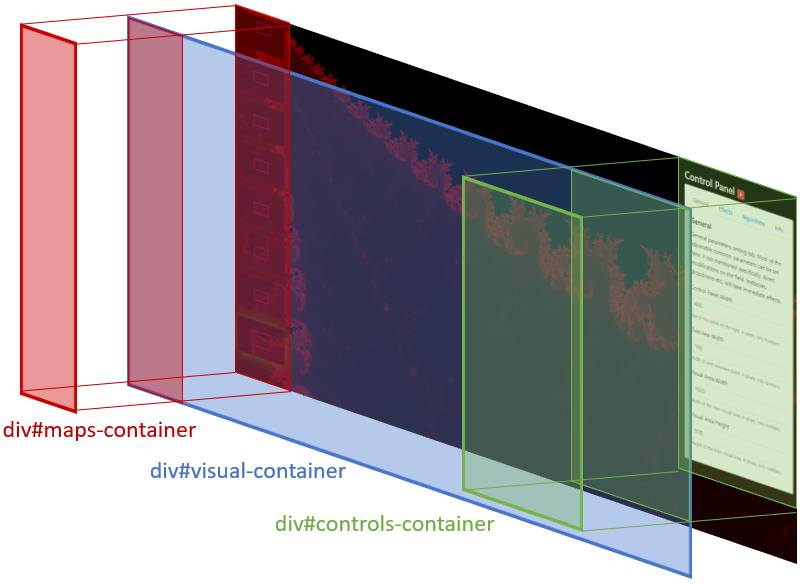
\includegraphics[width=\textwidth,keepaspectratio]{Figures/Chapter4/rootdom.png}
\decoRule
\caption[DOM Body Structure]{\gls{dom} structure in \texttt{<body>} tag.}
\label{fig:rootdom}
\end{figure}

After the visual \texttt{<div>} part, several \texttt{<script>} tags come after it to include what's necessary for the essential coding part. Here firstly are the dependencies of the project, including \emph{jQuery}, \emph{Bootstrap}'s \gls{js} part, and \emph{MiniBar}'s \gls{js} part. And then at the very end the main \gls{js} file \texttt{index.js} is included and all the core programs of this project goes in there.

Worth noting that conventionally all \gls{js} files should be included at the very end of the page as what we are doing now, unless the \gls{js} file is needed before the render phase of the web page. This way if the \gls{js} file is a little bit bigger than usual, the loading of the \gls{js} files won't affect the rendering process of the \gls{dom} documents.


\subsection{Main JavaScript \texttt{index.js}}

The main \gls{js} file \texttt{index.js} is where the core codes are. In this file there is firstly the definition of required classes from bottom level to the top, then the instantiation of them and putting the front end \gls{html} elements into action to display the overall results.

There in total four classes defined.

\subsubsection{Class \texttt{MandelWorker}}

The class \texttt{MandelWorker} is in charge of sending a message to the back end and when a result is sent back, handle it by executing a preset function(or say callback). This class is the red and green arrows shown in \gmref{fig:fpcpair}.

When instantiated, an instance of a native \emph{Web Worker} will also be created as a private property of this class. \texttt{MandelWorker} instantiates the \emph{Web Worker} by the script \texttt{naive\-worker.js}, which means that the script \texttt{naive\-worker.js} will be the core of the worker and this worker will be doing whatever in that script when it is asked to\footnote{ See \url{https://developer.mozilla.org/en-US/docs/Web/API/Web_Workers_API/Using_web_workers\#Spawning_a_dedicated_worker} for more detailed information of the process of instantiating a \emph{Web Worker}.}.

\textbf{Function \texttt{work(params...)}}

The function \texttt{work(params...)} is the interface between \texttt{MandelWorker} and the outside invoker. To get an image from the source, one must invoke this function with the needed parameters as follows:

\begin{itemize}
  \item \texttt{magnif} The magnification level of the result image to be expected from the \emph{Web Worker}.
  \item \texttt{centerX} The \texttt{x} component of the center coordinates on the mathmatical plane of the result image to be expected from the worker.
  \item \texttt{centerY} The \texttt{y} component of this coordinates.
  \item \texttt{width} The width in pixels of the result image.
  \item \texttt{height} The height in pixels of the result image.
  \item \texttt{callback} The function to execute when a result message is received.
  \item \texttt{callbackThis} The ``this'' context where the \texttt{callback} function should be executed under.
\end{itemize}

Here what's worth mentioning is the parameter \texttt{magnif}. The magnification level is a number representing the number of pixels that together has a length of $1$ on the mathmatical axis. As shown in \gmref{fig:magnif} is an image with the magnification level of $2$, since $2$ pixels have the length of $1$ on the mathmatical axis.

\begin{figure}[th]
\centering
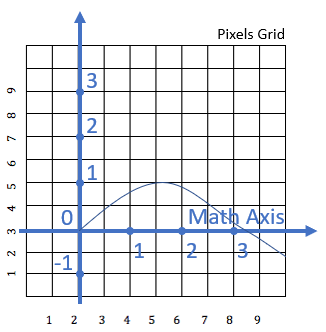
\includegraphics[keepaspectratio]{Figures/Chapter4/magnif.png}
\decoRule
\caption[Magnification Level]{Magnification level in aspect of mathmatical axis.}
\label{fig:magnif}
\end{figure}

Once this function is invoked, \texttt{MandelWorker} will tell its own \emph{Web Worker} to start working on datasets fetching\footnote{ In the context of the current project, is actually image generation. }, and if any sorts of results come through that worker, hit the \texttt{workerResponse(e)} function of the current \texttt{MandelWorker}.

\textbf{Function \texttt{workerResponse(e)}}

The function \texttt{workerResponse(e)} will be called when a response from the \emph{Web Worker} is sent back. It basically does one thing: checking if the parameters of \texttt{callback} and \texttt{callbackThis} were set when function \texttt{work(params...)} got invoked in the first place. If they were set to any function, call it under the conext of the parameter \texttt{callbackThis}.

\textbf{Function \texttt{destroy()}}

The function \texttt{destroy()} as the name implies is the method to destroy and release the resources for current \texttt{MandelWorker}. It terminates the \emph{Web Worker}, sets the response method to \texttt{null} so no responses will be dealt furthermore and sets all other references to \texttt{null} as well so the internal \gls{js} engine can garbage collect\footnote{ In computer science, garbage collection (GC) is a form of automatic memory management. The garbage collector, or just collector, attempts to reclaim garbage, or memory occupied by objects that are no longer in use by the program\cite{wiki:gc}.} all these instance to avoid memory leakage when the calculation gets heavy.

\subsubsection{Class \texttt{MapVisualPair}}

An abstract concept of pairing a minimap\footnote{ Same concept in current project as an \emph{overview}. } with an active focus region with higher resolution, as \gmref{fig:mapvisualpair} is an example of what they actually are respectively. This class is realizing the model of a pair of \gls{fpc} shown in \gmref{fig:fpcpair}.

\begin{figure}[th]
\centering
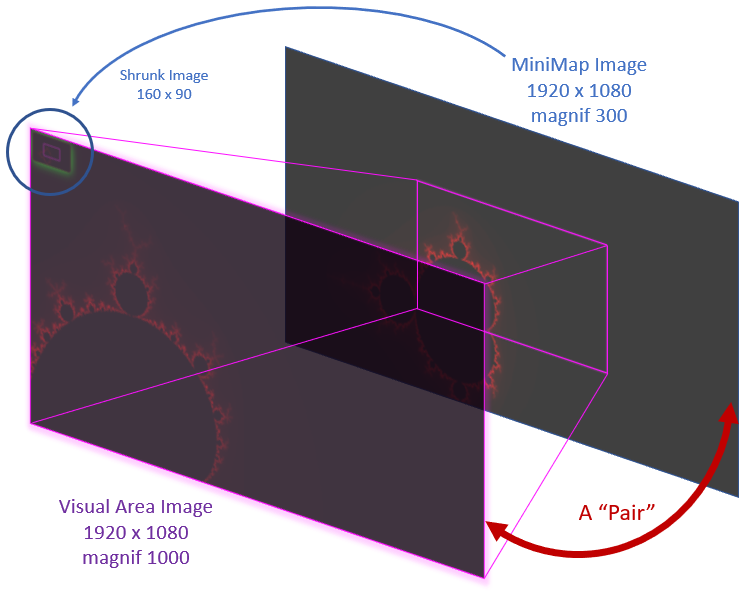
\includegraphics[width=\textwidth,keepaspectratio]{Figures/Chapter4/mapvisualpair.png}
\decoRule
\caption[Map Visual Pair]{Map area image and visual area(current focus region) image.}
\label{fig:mapvisualpair}
\end{figure}

The minimap representing a relatively ``larger'' area in the dataset and the visual area, which represents the active observing region, actually have both same resolution so they can both be displayed on a \gls{fhd} screen. Although the visual area seems ``smaller'' in comparison with the \gls{map} area, since it's an active region that is being observed by the user, the size of this visual area only represents its dimensions on the mathmatical plane and not smaller pixels-wise.

The \gls{map} image, however, will normally be shrunk and put on the left side of the screen, till the user hovers over a specific \gls{map} that will trigger the preview process of this program so he can have a glance of this image in a \gls{fhd} way.

The reason to pair up a visual area with a \gls{map} area is that whenever the user wants to browse around the dataset, the focusing coordinates on the visual area should also reflect back to the \gls{map} area, and the rectangle representing the current observing area should also get updated automatically. When there are more hierarchies of \glspl{map} present, this pairing mechanism becomes extremely helpful because the changes on the active region will flow all the way up to all levels of \glspl{map} necessary. Here \gmref{fig:mvp-pairflow} is a simple illustration of it.

\begin{figure}[th]
\centering
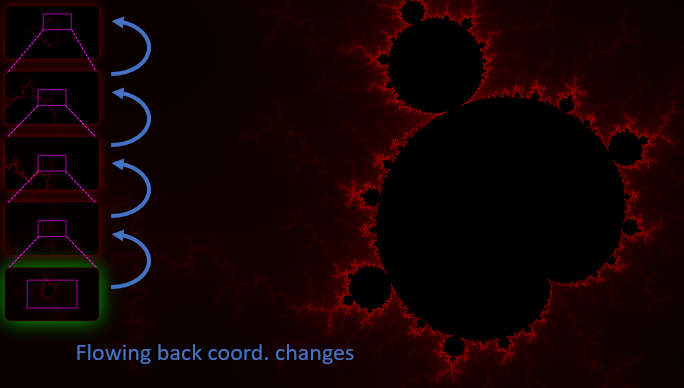
\includegraphics[width=\textwidth,keepaspectratio]{Figures/Chapter4/mvp-pairflow.png}
% 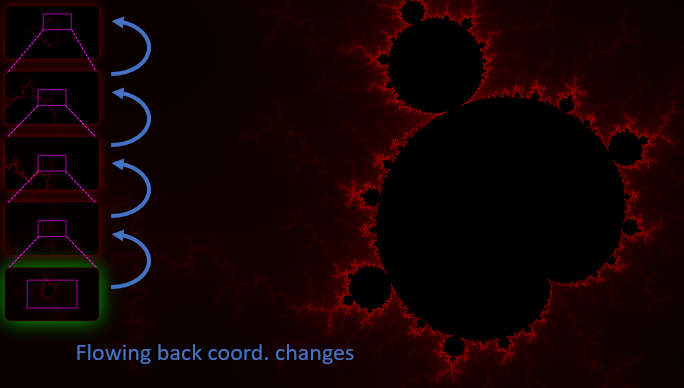
\includegraphics{Figures/Chapter4/mvp-pairflow.png}
\decoRule
\caption[Pairing Multiple Levels of \glspl{map}]{When multiple hierarchies of \glspl{map} present, visual area changes, all \glspl{map} changes.}
\label{fig:mvp-pairflow}
\end{figure}

\textbf{Function} \verb|init(mapCanvas, previewCanvas, visCanvas = null)|

This function will initialize the current \texttt{MapVisualPair}, bounding a \texttt{mapCanvas}, a \texttt{previewCanvas} and a \texttt{visCanvas} all of type \texttt{<canvas>} element to this class. When internally a drawing action should be performed, related images will be drawn on corresponding canvas.

The canvas \texttt{mapCanvas} will be used to draw the shrunk version of the \gls{map} image. \texttt{previewCanvas} will be used to draw the normal(\gls{fhd}) version of the \gls{map} image. And \texttt{visCanvas} will be used to draw the visual area image in \gls{fhd} if set.

After bounding the canvases, this function will also check if any event handlers are bound to the events \texttt{mouseover} and \texttt{mouseout} to the \texttt{mapCanvas} element, and record corresponding info to the element to avoid attemps to rebound event handlers to the same \texttt{<canvas>} element. In this way, only one event handler for \texttt{mouseover} and \texttt{mouseout} will be triggered when the user hovers their mouse on the \texttt{<canvas>} and when the user put their cursor out of the element.

The handlers this function is going to bound to the \texttt{mapCanvas} element are going to first add \gls{css} class \texttt{.nearby} to adjacent siblings of this canvas, and check if any additional callbacks this class should call. The callbacks, if any, which are set in the private properties \texttt{mouseOverCallback} and \texttt{mouseOutCallback}, will be called under set context \texttt{mouseOverCallbackThis} and \texttt{mouseOutCallbackThis} when user performs corresponding actions. As mentioned before, they will also be called only once because the bounding information is recorded. In the project, these callbacks and the contexts of them are set by a manager class \gmref{chap4:effectmanager}.

\textbf{Function} \verb|destroy()|

This function as the name implies releases all in-use resources, including \texttt{Worker}s, unbinding bound event handlers, clearing references to the canvases and their 2d contexts.

\textbf{Function} \verb|drawMapHoverArea(offsetRealX = 0, offsetRealY = 0)|

When the class is told to draw images on corresponding canvas elements, it will not automatically draw the purple rectangle indicating the current observing visual area, since the cached image data does not include this rectangle --- it doesn't belong to the extreme resolution dataset itself, therefore, this function exists to draw this current focus area using a purple rectangle to indicate it, drawing this rectangle on the \texttt{mapCanvas} whenever invoked. Note that whenever the image from the calculation side is fetched, without invoking this function, no current obeserving area rectangle will be shown, since the newly fetched image data will cover the old one also the old drawn rectangle.

The parameters \texttt{offsetRealX} and \texttt{offsetRealY} can also be set, as the purple rectangle to be drawn will then have an offset of (\texttt{offsetRealX}, \texttt{offsetRealY}) with respect to the center of the current observing area on the mathmatical complex plane.

\textbf{Function} \verb|drawPreviewHoverArea(offsetRealX = 0, offsetRealY = 0)|

Like the function \texttt{drawMapHoverArea}, this function will also draw a rectangle representing the current observing visual area, but on another canvas \texttt{previewCanvas}. The reason to separate these two functions is that the canvas \texttt{previewCanvas} isn't always visible and if these two functions are combined, it'll draw unintended purple rectangles on wrong canvases.

\textbf{Function} \verb|moveTo(x = null, y = null)|

This function is used to move the current \texttt{MapVisualPair} around. The parameters of coordinates are on the mathmatical complex plane, i.e. with respect to the entire datasets.

Note that these two parameters can be omitted and when omitted, the current \texttt{MapVisualPair} will simply send a ping to the calculation side and grab new image data for current observing coordinates, like a ``refresh'' action.

\textbf{Properties} \texttt{visMagnif} and \texttt{mapMagnif}

The magnification for the pair of these two canvases. See \gmref{fig:magnif} for the explanation of magnification level.

\textbf{Properties} \texttt{visCenterX} and \texttt{visCenterY}

The coordinates of the center point of the current observing visual area, with respect to the mathmatical complex plane.

\textbf{Properties} \texttt{visCanvasWidth} and \texttt{visCanvasHeight}

The width and height in \textbf{pixels} of the image data of the whole visual area. In \gmref{fig:mapvisualpair}, they're the dimensions of the whole visual area image. These properties have to exist because the dimensions of this area cannot always be fetched from the \texttt{visCanvas} property, as it is an optional parameter during the \texttt{init(params..)} phase and sometimes is absent.

\textbf{Properties} \texttt{visImgOffsetX} and \texttt{visImgOffsetY}

These two properties are set for the dragging actions that are realized in \gmref{chap4:minimapmanager}. They represents the current dragging offset with respect to the top left corner of the \texttt{visCanvas}. The reference point being top left corner not the center point is because in web canvas drawing system, the (0, 0) point is the top left corner, unlike in mathmatical complex plane it being the center.

\textbf{Properties} \texttt{mapCenterX} and \texttt{mapCenterY}

Like the properties \texttt{visCenterX} and \texttt{visCenterY}, these two properties represents the coordinates of the center point of the current \gls{map} area, with respect to the mathmatical complex plane. In \gmref{fig:mapvisualpair}, they're the center coordinates of the \gls{map} image.

\subsubsection{Class \texttt{MinimapManager}}\label{chap4:minimapmanager}

The manager class of all the minimaps, controlling all their behaviours on the top level. This class is described in \gmref{fig:fpcmanager}, the manager of all the \gls{fpc} models, plus a \gls{fhd} visual area.

\textbf{Inits}

\textbf{Function} \path{initMaps(visCanvas, previewCanvas, mapsContainer, visualContain er, hoverX = 0, hoverY = 0)}

This function initializes the states of all the \texttt{MapVisualPair}s that should be displayed, as well as initializing its own requird properties.

The properties \texttt{visCanvas} and \texttt{previewCanvas} are the canvases bound to this manager. \texttt{visCanvas} is the canvas for the main visual area and the details image is rendered on this canvas. \texttt{previewCanvas} is the canvas that's initially hidden, but will be shown when the \texttt{EffectManager} described in \gmref{chap4:effectmanager} instructs, designed for the presentation of the preview images. These two canvases have exactly the same dimensions, covering the entire \gls{ui} viewport, and on the most bottom layer of the page hence being laid over by the \glspl{map} and control panels. \texttt{previewCanvas} in turn lays over \texttt{visCanvas} since when a preview instruction is issued, it has to be displayed over the original visual area.

The property \texttt{mapsContainer} is the container holding all the canvases for the display of \glspl{map}. It's bound to this manager during this initialization phase. During this phase, step one, basic \gls{dom} structure of one \gls{map}, consisting of one \texttt{<cavans>} element and one \texttt{<span>} element for the purpose of showing the \texttt{magnif} number, will be created and appended to this container. The center coordinates of the \gls{map} will be from the parameters \texttt{hoverX} and \texttt{hoverY}, and \texttt{0} if not designated. The \texttt{magnif} level of the first \gls{map} comes from the variable \texttt{mapMagnif} in the global scope of \texttt{index.js}\footnote{ Technically not the global scope of entire \texttt{index.js} file per se, but the ``global scope'' of entire anonymous function that envelops all the codes.}. Based on the \texttt{magnif} of the first \gls{map} and the \texttt{visMagnif} variable defined in global scope, the initial dimensions of the focus area projected on the \gls{map} can be calculated.

With the dimensions of the first \gls{map}, this manager then decides whether additional \glspl{map} are required, based on the results of whether this projected area on \gls{map} is too small. If this area is too small, additional \gls{dom} structure consisting of one \texttt{<canvas>} and one \texttt{<span>} will be created and appended to the container. The criteria of whether this area is too small is defined by the private property \texttt{this.minStrokeW}\footnote{ In pixels.} of this manager. After the new \gls{dom} is created, we then will have two canvases. The first one will be the \gls{map} canvas and the one created after the calculation of the projection area will be the ``visual'' area. These two areas will then be paired up, forming an object of \texttt{MapVisualPair}. The \texttt{magnif} value of the visual area will be determined by the \texttt{magnif} value of the \gls{map} area, the minimal dimensions allowed for the projection area preset in \texttt{this.minStrokeW} and the dimensions of the dimensions of \texttt{previewCanvas}.

Since the model of \gls{fpc} are hierarchical, we can easily see that the new \texttt{magnif} value of the next \gls{map} area will be the value of the \texttt{magnif} value of the previous visual area. After the pairing of these two \glspl{map} and forming a first \texttt{MapVisualPair}, we can repeat this process described in above paragraph until the projection area on the current \gls{map} area is big enough then set in \texttt{this.minStrokeW}. When this happens, we bind the most recent \gls{map} canvas with the main visual area canvas and form the final \texttt{MapVisualPair}. This pair is named \texttt{this.pairMain} in this manager.

And the end of the initialization process, we put all these generated \texttt{MapVisualPair}s in an array called \texttt{this.pairs} and also bind \texttt{visualContainer} which holds \texttt{visCanvas} and \texttt{previewCanvas} with this manager. Later this container will be used for the events binding of \gls{ui} interactions.

\textbf{Function} \verb|initPairMainDrag()|

This function is called after the process in \texttt{initMaps(params..)} is complete. It registers necessary event handlers for mouse dragging related events that allows for browsing around the center of the focus view like Google Maps, including:

\begin{itemize}
  \item \path{pairMainMouseDown(e)} is bound with what was set in \texttt{visContainer} property, responding to single mouse pressing event without releasing the button.
  \item \path{pairMainMouseMove(e)} is bound with what was set in \texttt{visContainer} property, responding to single mouse moving event without releasing the button.
  \item \path{pairMainMouseUp(e)} is bound with what was set in properties \texttt{visContainer} \textbf{or} anywhere on the web page, responding to single mouse button releasing event.
\end{itemize}

All the handlers are bound under the context of the current class, a.k.a \texttt{this} or \texttt{MinimapManager}.

\textbf{Function} \verb|initPairMainWheel()|

This function can be called after the process in \texttt{initMaps(params..)} is complete. In the project it is called after \texttt{initPairMainDrag()}. It registers necessary event handlers for mouse wheeling related events that allows zooming into the dataset on the fly like Google Maps. It binds the event handler \texttt{pairMainWheel(e)} to the mouse wheel event with the root document of the web page, which means when user tries to scroll the middle button of thier mouse, this handler will be triggered.

This handler is also bound under the context of the current class, a.k.a \texttt{this} or \texttt{MinimapManager}.

\textbf{Handlers and Functions Related with Mouse Dragging}

\textbf{Function} \path{pairMainMouseDown(e)}

As mentioned before, this function handles the event when user presses the left mouse button before releasing it.

When this event happens on the target, we first records the current position of the user's cursor on the attributes \texttt{dragStartX}, \texttt{dragStartY}, \texttt{dragCurrentMouseX} and \texttt{dragCurrentMouseY}, and use \texttt{window.requestAnimationFrame(callback)} to activate an animation with max frame rates allowed. The \texttt{callback} parameter in \path{window.requestAnimationFrame(callback)} is the method \texttt{pairMainStepDrag(timestamp)} of this manager and will be called every time when a new frame should be rendered to the screen and we use this mechanism to repaint the dragged image of the current focus area in the correct place.

This function also sets a \texttt{dragGlobalID} property to the class to mark that this process has been marked started.

\textbf{Function} \path{pairMainMouseMove(e)}

This function handles the situation when the user, while not releasing the left mouse button, moves the mouse around.

This function does one simple thing: if the \texttt{dragGlobalID} attribute is set on the class meaning the process of mouse dragging being started, set the current postion of user's cursor to the attributes \texttt{dragCurrentMouseX} and \texttt{dragCurrentMouseY} to be used by \texttt{pairMainStepDrag(timestamp)}.

\textbf{Function} \path{pairMainStepDrag(timestamp)}

During the phase of dragging, since this function is triggered every time a new frame is needed to be rendered, we simply grab the values in \texttt{dragCurrentMouseX} and \texttt{dragCurrentMouseY}, and compare them with \texttt{dragStartX} and \texttt{dragStartY}, and see how much the user has moved their mouse since the last frame rendered.

We then paint the image based on the offsets we calculated from these two pairs of values on the correct position.

\textbf{Function} \path{pairMainMouseUp(e)}

When user releases the mouse button after the series of the previous events, this handler gets triggered.

We repaint the image of the focus area one last time on the correct place, and put this final offset on the properties \texttt{visImgOffsetX} and \texttt{visImgOffsetY} of \texttt{this.pairMain}, and stop the animation using \texttt{window.cancelAnimationFrame(this.dragGlobalID)} with the help of the recorded \texttt{dragGlobalID}.

At this point, new coordinates of the current center of visual view will be calculated and check how many of the \texttt{MapVisualPair}s need updates. All of those that need updates will be instructed to send requests to back end resolver and fetch new image data.

The properties \texttt{visImgOffsetX} and \texttt{visImgOffsetY} are set on \texttt{this.pairMain} so next time when user starts to drag the mouse, the image of the visual area will start from the current offset and not jump back to the initial offset of this drag which is \texttt{(0, 0)}, even if the calculation from the resolver hasn't completed yet. This mechanism can be compared with this situation of Google Maps: when user is looking at location $A$ and the loading is completed, and drags the map around and stops at another location $B$, the map will start to fetch the data around location $B$. However, if the user refuses to wait and starts to drag again to a new location $C$, the second drag starts from location $B$ and not location $A$.

\textbf{Handlers and Functions Related with Zooming In and Out}

\textbf{Function} \path{pairMainWheel(e)}

This function handles the event when user scrolls the middle button of their mouse.

In this handler, we first check if this process is already ongoing or not.

If this process hasn't been started yet, we set a property \texttt{wheelCurrentRatio} representing how much user has zoomed in to \texttt{1}, and records the current \texttt{magnif} value of the visual area, \texttt{visMagnif}. We then request a same rendering mechanism trigger by \texttt{window.requestAnimationFrame} and pass on the frame executor \path{pairMainStepWheel (timestamp)} to start an animation for zooming in. After that, while the zooming animation of the current visual area image is ongoing, we set a timer of $500$ milliseconds that detects if the scrolling on the mouse button is still happening. When the timer hits, meaning within $500$ milliseconds the user hasn't scrolled the mouse button, we should consider that user wants to stop the zooming at current depth.

If this process is started already, meaning this process is still ongoing, we only refresh the counter of the timer, and reset it back to $500$ milliseconds and let the \texttt{pairMainStepWheel(timestamp)} to keep working on each frames of the animation.

\textbf{Function} \path{pairMainStepWheel()}

During the phase of zooming in or out of the dataset, this function is triggered every time a new frame is needed to be rendered. We check if the zooming direction is in or out, then repaint the zoomed image and calculate the new \texttt{visMagnif}\footnote{ As mentioned before, the \texttt{magnif} value of the main visual area.}.

\textbf{Function} \path{pairMainTimeoutWheel()}

If this function gets triggered, it means the timer has timed out and user wants to stop at current depth. Since each frame we have the value of \texttt{visMagnif} calculated, we now have a new \texttt{magnif} value for the visual area in the system. 

To make the current system has the clear resolution again, two situation can happen: user has either zoomed deeper into the dataset, or has zoomed out shallower.

When the first situation is the case, we start from the most zoomed in \gls{map}, and check whether with its \texttt{magnif} value new \glspl{map} are needed. This process is the same as described in \texttt{initMaps(params...)} since we're here also initializing new \glspl{map}, adding more to the pile of \texttt{this.pairs}.

When the second situation is the case, we do the reverse way of the initializing process. If the current projection area is larger than the most zoomed in \gls{map} entirely, this \gls{map} is no longer needed and needs to be removed. We delete this \gls{map}, invoking all the \texttt{destroy()} methods on \texttt{MapVisualPair} and their \texttt{MandelWorker}s, and move one level upper. We stop at the level where the projection area is small enough within one \gls{map}, and reconnect the current most zoomed in map with the canvas of the main visual area.

After the increment or decrement of the \glspl{map}, \texttt{MapVisualPair} that needs to get updates will be instructed to send requests to resolvers.

\subsubsection{Class \texttt{EffectManager}}\label{chap4:effectmanager}

This class manages the behaviours, activation and deactivation of the overview effects and the preview effects of the overviews.

General functions: \texttt{init()}, \texttt{getInfo(el)}

Fade in / out related functions: \texttt{fadeMouseOver(e, currentPair)}, \texttt{fadeMouseOut(e, currentPair)}

Zoom in / out through related functions: \texttt{zoomMouseOver(e, currentPair)}, \texttt{zoomStep(timestamp)}, \texttt{zoomMouseOut(e, currentPair)}

General preview effects functions: \texttt{updatePreview()}, \texttt{updateFadePreview()}, \texttt{updateZoomPreview()}, \texttt{destroyPreview()}

General overview effects functions: \texttt{destroy()}, \texttt{update()}

Scrollbar + Dock effects specific functions: \texttt{initScrollbar()}, \texttt{destroyScrollbar()}, \texttt{updateScrollbar()}

Stacked Cards effects specific functions: \texttt{initStacked()}, \texttt{destroyStacked()}, \texttt{updateStacked()}

Tabs effects specific functions: \texttt{initTabs()}, \texttt{destroyTabs()}, \texttt{updateTabs()}

\subsubsection{Instantiation, Variables and the Rest}

\begin{itemize}
  \item \texttt{screenWidth}
  \item \texttt{screenHeight}
  \item \texttt{mapWidth}
  \item \texttt{mapHeight}
  \item \texttt{controlPanelWidth}
  \item \texttt{visMagnif}
  \item \texttt{mapMagnif}
  \item \texttt{hoverX}
  \item \texttt{hoverY}
  \item \texttt{mainCanvas}
  \item \texttt{previewCanvas}
  \item \texttt{\$(`\#visual-container')}
  \item \texttt{\$(`\#maps-container')}
\end{itemize}

\subsection{CSSs for Overview Effects}
\label{chap4:frontend-css}

Folder \texttt{./css} includes five \gls{css} files, each setting up some visual effects of the project.

File \texttt{./css/common.css} first sets up all general appearance of the elements on the web page when no parameters or effects are set. File \texttt{./css/dock.css} sets up the appearance when \emph{Scrollbar + Dock} is activated, only the iOS Dock part and file \\\texttt{./css/minibar.css} sets up the scroll bar part. File \texttt{./css/stacked.css} sets up the effects of stacked cards. File \texttt{./css/tabs.css} sets up the effects of the tab selection on the top.

\subsection{Scrollbar + Dock Effect}

\subsection{Stacked Cards Effect}

\subsection{Tabs Effect}

%----------------------------------------------------------------------------------------
%	SECTION 
%----------------------------------------------------------------------------------------

\section{Back End Calculation}

The back end calculation is done in the \gls{js} file \texttt{naive-worker.js}. This file is being used for initializing the \emph{WebWorker}s inside \texttt{index.js} dynamically. Whenever a calculation or extraction for a specific region of a dataset is needed, the main \gls{js} file \texttt{index.js} is going to send a message to \texttt{naive-worker.js} with desired parameters and this back end will respond with corresponding image data.

\begin{figure}[th]
\centering
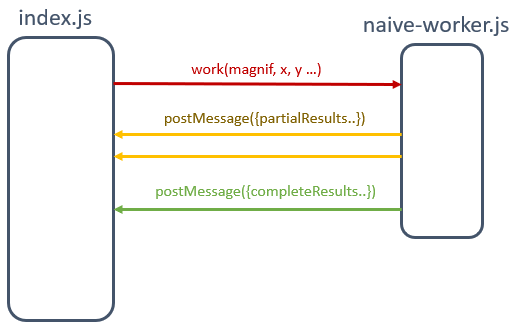
\includegraphics{Figures/Chapter4/messageexchange.png}
\decoRule
\caption[Message Exchange]{Message exchange between \texttt{index.js} and \texttt{naive-worker.js}.}
\label{fig:messageexchange}
\end{figure}

\subsection{Global Scope}

In the global scope of this file, the following things were done.

\paragraph{Includes} The \texttt{decimal.js} dependency is included for high-precision floating points calculation. Default parameters for the dependency is set.

\paragraph{Constants} Constants of default screen width and default screen height are defined in case the front end doesn't give these parameters.

\paragraph{Canvas} An \texttt{OffscreenCanvas} instance is created and instantiated with the dimensions of by default the values of the defined constants. The \texttt{OffscreenCanvas} will be used as the canvas to generate the desired image on, and since it's not being shown on the screen, will occupy less system resources and boost the calculation speed. Corresponding variables is declared after the instantiation, respectively \texttt{canvas} for the \texttt{OffscreenCanvas} itself and \texttt{ctx} as the 2d context of the canvas.

\subsection{Message Reception}

See \gmref{fig:messageexchange}.

\subsection{Iteration Limit}

\subsection{Iteration Count for One Point}

\subsection{Image Generation}

\subsection{High Precision Version}

%----------------------------------------------------------------------------------------
%	SECTION 
%----------------------------------------------------------------------------------------

\section{Utility Assets}

Other open source third-party utilities lie in different folders with corresponding names.

\subsection{Folder \texttt{./js}}

In \texttt{./js} folder, all \gls{js} third-party files are here, including:

\begin{itemize}
    \item File \texttt{decimal.min.js} is for high-precision floating points calculation for \acrfull{js}.
    \item File \texttt{jquery-3.4.1.min.js} is for \gls{dom} traversal and manipulation, event handling and animation.
    \item File \texttt{bootstrap.bundle.min.js} is for some basic styling of the control panel sitting on top right corner of the screen.
\end{itemize}

\subsection{Folder \texttt{./fa}}

\subsection{Folder \texttt{./bs}}

\subsection{Folder \texttt{./css}}
% Chapter Template

\chapter{Results and Comparison} % Main chapter title

\label{Chapter5} % Change X to a consecutive number; for referencing this chapter elsewhere, use \ref{ChapterX}

%----------------------------------------------------------------------------------------
%	SECTION
%----------------------------------------------------------------------------------------

\section{General Results}

%----------------------------------------------------------------------------------------
%	SECTION
%----------------------------------------------------------------------------------------

\section{Comparison Between Different Arrangement Methods}

%----------------------------------------------------------------------------------------
%	SECTION
%----------------------------------------------------------------------------------------

\section{Future Work}
% % Chapter 1

\chapter{Chapter Title Here} % Main chapter title

\label{ChapterRef} % For referencing the chapter elsewhere, use \ref{Chapter1} 

%----------------------------------------------------------------------------------------

% Define some commands to keep the formatting separated from the content 
\newcommand{\keyword}[1]{\textbf{#1}}
\newcommand{\tabhead}[1]{\textbf{#1}}
\newcommand{\code}[1]{\texttt{#1}}
\newcommand{\file}[1]{\texttt{\bfseries#1}}
\newcommand{\option}[1]{\texttt{\itshape#1}}

%----------------------------------------------------------------------------------------

\section{Welcome and Thank You}
Welcome to this \LaTeX{} Thesis Template, a beautiful and easy to use template for writing a thesis using the \LaTeX{} typesetting system.

If you are writing a thesis (or will be in the future) and its subject is technical or mathematical (though it doesn't have to be), then creating it in \LaTeX{} is highly recommended as a way to make sure you can just get down to the essential writing without having to worry over formatting or wasting time arguing with your word processor.

\LaTeX{} is easily able to professionally typeset documents that run to hundreds or thousands of pages long. With simple mark-up commands, it automatically sets out the table of contents, margins, page headers and footers and keeps the formatting consistent and beautiful. One of its main strengths is the way it can easily typeset mathematics, even \emph{heavy} mathematics. Even if those equations are the most horribly twisted and most difficult mathematical problems that can only be solved on a super-computer, you can at least count on \LaTeX{} to make them look stunning.

%----------------------------------------------------------------------------------------

\section{Learning \LaTeX{}}

\LaTeX{} is not a \textsc{wysiwyg} (What You See is What You Get) program, unlike word processors such as Microsoft Word or Apple's Pages. Instead, a document written for \LaTeX{} is actually a simple, plain text file that contains \emph{no formatting}. You tell \LaTeX{} how you want the formatting in the finished document by writing in simple commands amongst the text, for example, if I want to use \emph{italic text for emphasis}, I write the \verb|\emph{text}| command and put the text I want in italics in between the curly braces. This means that \LaTeX{} is a \enquote{mark-up} language, very much like HTML.

\subsection{A (not so short) Introduction to \LaTeX{}}

If you are new to \LaTeX{}, there is a very good eBook -- freely available online as a PDF file -- called, \enquote{The Not So Short Introduction to \LaTeX{}}. The book's title is typically shortened to just \emph{lshort}. You can download the latest version (as it is occasionally updated) from here:
\url{http://www.ctan.org/tex-archive/info/lshort/english/lshort.pdf}

It is also available in several other languages. Find yours from the list on this page: \url{http://www.ctan.org/tex-archive/info/lshort/}

It is recommended to take a little time out to learn how to use \LaTeX{} by creating several, small `test' documents, or having a close look at several templates on:\\ 
\url{http://www.LaTeXTemplates.com}\\ 
Making the effort now means you're not stuck learning the system when what you \emph{really} need to be doing is writing your thesis.

\subsection{A Short Math Guide for \LaTeX{}}

If you are writing a technical or mathematical thesis, then you may want to read the document by the AMS (American Mathematical Society) called, \enquote{A Short Math Guide for \LaTeX{}}. It can be found online here:
\url{http://www.ams.org/tex/amslatex.html}
under the \enquote{Additional Documentation} section towards the bottom of the page.

\subsection{Common \LaTeX{} Math Symbols}
There are a multitude of mathematical symbols available for \LaTeX{} and it would take a great effort to learn the commands for them all. The most common ones you are likely to use are shown on this page:
\url{http://www.sunilpatel.co.uk/latex-type/latex-math-symbols/}

You can use this page as a reference or crib sheet, the symbols are rendered as large, high quality images so you can quickly find the \LaTeX{} command for the symbol you need.

\subsection{\LaTeX{} on a Mac}
 
The \LaTeX{} distribution is available for many systems including Windows, Linux and Mac OS X. The package for OS X is called MacTeX and it contains all the applications you need -- bundled together and pre-customized -- for a fully working \LaTeX{} environment and work flow.
 
MacTeX includes a custom dedicated \LaTeX{} editor called TeXShop for writing your `\file{.tex}' files and BibDesk: a program to manage your references and create your bibliography section just as easily as managing songs and creating playlists in iTunes.

%----------------------------------------------------------------------------------------

\section{Getting Started with this Template}

If you are familiar with \LaTeX{}, then you should explore the directory structure of the template and then proceed to place your own information into the \emph{THESIS INFORMATION} block of the \file{main.tex} file. You can then modify the rest of this file to your unique specifications based on your degree/university. Section \ref{FillingFile} on page \pageref{FillingFile} will help you do this. Make sure you also read section \ref{ThesisConventions} about thesis conventions to get the most out of this template.

If you are new to \LaTeX{} it is recommended that you carry on reading through the rest of the information in this document.

Before you begin using this template you should ensure that its style complies with the thesis style guidelines imposed by your institution. In most cases this template style and layout will be suitable. If it is not, it may only require a small change to bring the template in line with your institution's recommendations. These modifications will need to be done on the \file{MastersDoctoralThesis.cls} file.

\subsection{About this Template}

This \LaTeX{} Thesis Template is originally based and created around a \LaTeX{} style file created by Steve R.\ Gunn from the University of Southampton (UK), department of Electronics and Computer Science. You can find his original thesis style file at his site, here:
\url{http://www.ecs.soton.ac.uk/~srg/softwaretools/document/templates/}

Steve's \file{ecsthesis.cls} was then taken by Sunil Patel who modified it by creating a skeleton framework and folder structure to place the thesis files in. The resulting template can be found on Sunil's site here:
\url{http://www.sunilpatel.co.uk/thesis-template}

Sunil's template was made available through \url{http://www.LaTeXTemplates.com} where it was modified many times based on user requests and questions. Version 2.0 and onwards of this template represents a major modification to Sunil's template and is, in fact, hardly recognisable. The work to make version 2.0 possible was carried out by \href{mailto:vel@latextemplates.com}{Vel} and Johannes Böttcher.

%----------------------------------------------------------------------------------------

\section{What this Template Includes}

\subsection{Folders}

This template comes as a single zip file that expands out to several files and folders. The folder names are mostly self-explanatory:

\keyword{Appendices} -- this is the folder where you put the appendices. Each appendix should go into its own separate \file{.tex} file. An example and template are included in the directory.

\keyword{Chapters} -- this is the folder where you put the thesis chapters. A thesis usually has about six chapters, though there is no hard rule on this. Each chapter should go in its own separate \file{.tex} file and they can be split as:
\begin{itemize}
\item Chapter 1: Introduction to the thesis topic
\item Chapter 2: Background information and theory
\item Chapter 3: (Laboratory) experimental setup
\item Chapter 4: Details of experiment 1
\item Chapter 5: Details of experiment 2
\item Chapter 6: Discussion of the experimental results
\item Chapter 7: Conclusion and future directions
\end{itemize}
This chapter layout is specialised for the experimental sciences, your discipline may be different.

\keyword{Figures} -- this folder contains all figures for the thesis. These are the final images that will go into the thesis document.

\subsection{Files}

Included are also several files, most of them are plain text and you can see their contents in a text editor. After initial compilation, you will see that more auxiliary files are created by \LaTeX{} or BibTeX and which you don't need to delete or worry about:

\keyword{example.bib} -- this is an important file that contains all the bibliographic information and references that you will be citing in the thesis for use with BibTeX. You can write it manually, but there are reference manager programs available that will create and manage it for you. Bibliographies in \LaTeX{} are a large subject and you may need to read about BibTeX before starting with this. Many modern reference managers will allow you to export your references in BibTeX format which greatly eases the amount of work you have to do.

\keyword{MastersDoctoralThesis.cls} -- this is an important file. It is the class file that tells \LaTeX{} how to format the thesis. 

\keyword{main.pdf} -- this is your beautifully typeset thesis (in the PDF file format) created by \LaTeX{}. It is supplied in the PDF with the template and after you compile the template you should get an identical version.

\keyword{main.tex} -- this is an important file. This is the file that you tell \LaTeX{} to compile to produce your thesis as a PDF file. It contains the framework and constructs that tell \LaTeX{} how to layout the thesis. It is heavily commented so you can read exactly what each line of code does and why it is there. After you put your own information into the \emph{THESIS INFORMATION} block -- you have now started your thesis!

Files that are \emph{not} included, but are created by \LaTeX{} as auxiliary files include:

\keyword{main.aux} -- this is an auxiliary file generated by \LaTeX{}, if it is deleted \LaTeX{} simply regenerates it when you run the main \file{.tex} file.

\keyword{main.bbl} -- this is an auxiliary file generated by BibTeX, if it is deleted, BibTeX simply regenerates it when you run the \file{main.aux} file. Whereas the \file{.bib} file contains all the references you have, this \file{.bbl} file contains the references you have actually cited in the thesis and is used to build the bibliography section of the thesis.

\keyword{main.blg} -- this is an auxiliary file generated by BibTeX, if it is deleted BibTeX simply regenerates it when you run the main \file{.aux} file.

\keyword{main.lof} -- this is an auxiliary file generated by \LaTeX{}, if it is deleted \LaTeX{} simply regenerates it when you run the main \file{.tex} file. It tells \LaTeX{} how to build the \emph{List of Figures} section.

\keyword{main.log} -- this is an auxiliary file generated by \LaTeX{}, if it is deleted \LaTeX{} simply regenerates it when you run the main \file{.tex} file. It contains messages from \LaTeX{}, if you receive errors and warnings from \LaTeX{}, they will be in this \file{.log} file.

\keyword{main.lot} -- this is an auxiliary file generated by \LaTeX{}, if it is deleted \LaTeX{} simply regenerates it when you run the main \file{.tex} file. It tells \LaTeX{} how to build the \emph{List of Tables} section.

\keyword{main.out} -- this is an auxiliary file generated by \LaTeX{}, if it is deleted \LaTeX{} simply regenerates it when you run the main \file{.tex} file.

So from this long list, only the files with the \file{.bib}, \file{.cls} and \file{.tex} extensions are the most important ones. The other auxiliary files can be ignored or deleted as \LaTeX{} and BibTeX will regenerate them.

%----------------------------------------------------------------------------------------

\section{Filling in Your Information in the \file{main.tex} File}\label{FillingFile}

You will need to personalise the thesis template and make it your own by filling in your own information. This is done by editing the \file{main.tex} file in a text editor or your favourite LaTeX environment.

Open the file and scroll down to the third large block titled \emph{THESIS INFORMATION} where you can see the entries for \emph{University Name}, \emph{Department Name}, etc \ldots

Fill out the information about yourself, your group and institution. You can also insert web links, if you do, make sure you use the full URL, including the \code{http://} for this. If you don't want these to be linked, simply remove the \verb|\href{url}{name}| and only leave the name.

When you have done this, save the file and recompile \code{main.tex}. All the information you filled in should now be in the PDF, complete with web links. You can now begin your thesis proper!

%----------------------------------------------------------------------------------------

\section{The \code{main.tex} File Explained}

The \file{main.tex} file contains the structure of the thesis. There are plenty of written comments that explain what pages, sections and formatting the \LaTeX{} code is creating. Each major document element is divided into commented blocks with titles in all capitals to make it obvious what the following bit of code is doing. Initially there seems to be a lot of \LaTeX{} code, but this is all formatting, and it has all been taken care of so you don't have to do it.

Begin by checking that your information on the title page is correct. For the thesis declaration, your institution may insist on something different than the text given. If this is the case, just replace what you see with what is required in the \emph{DECLARATION PAGE} block.

Then comes a page which contains a funny quote. You can put your own, or quote your favourite scientist, author, person, and so on. Make sure to put the name of the person who you took the quote from.

Following this is the abstract page which summarises your work in a condensed way and can almost be used as a standalone document to describe what you have done. The text you write will cause the heading to move up so don't worry about running out of space.

Next come the acknowledgements. On this page, write about all the people who you wish to thank (not forgetting parents, partners and your advisor/supervisor).

The contents pages, list of figures and tables are all taken care of for you and do not need to be manually created or edited. The next set of pages are more likely to be optional and can be deleted since they are for a more technical thesis: insert a list of abbreviations you have used in the thesis, then a list of the physical constants and numbers you refer to and finally, a list of mathematical symbols used in any formulae. Making the effort to fill these tables means the reader has a one-stop place to refer to instead of searching the internet and references to try and find out what you meant by certain abbreviations or symbols.

The list of symbols is split into the Roman and Greek alphabets. Whereas the abbreviations and symbols ought to be listed in alphabetical order (and this is \emph{not} done automatically for you) the list of physical constants should be grouped into similar themes.

The next page contains a one line dedication. Who will you dedicate your thesis to?

Finally, there is the block where the chapters are included. Uncomment the lines (delete the \code{\%} character) as you write the chapters. Each chapter should be written in its own file and put into the \emph{Chapters} folder and named \file{Chapter1}, \file{Chapter2}, etc\ldots Similarly for the appendices, uncomment the lines as you need them. Each appendix should go into its own file and placed in the \emph{Appendices} folder.

After the preamble, chapters and appendices finally comes the bibliography. The bibliography style (called \option{authoryear}) is used for the bibliography and is a fully featured style that will even include links to where the referenced paper can be found online. Do not underestimate how grateful your reader will be to find that a reference to a paper is just a click away. Of course, this relies on you putting the URL information into the BibTeX file in the first place.

%----------------------------------------------------------------------------------------

\section{Thesis Features and Conventions}\label{ThesisConventions}

To get the best out of this template, there are a few conventions that you may want to follow.

One of the most important (and most difficult) things to keep track of in such a long document as a thesis is consistency. Using certain conventions and ways of doing things (such as using a Todo list) makes the job easier. Of course, all of these are optional and you can adopt your own method.

\subsection{Printing Format}

This thesis template is designed for double sided printing (i.e. content on the front and back of pages) as most theses are printed and bound this way. Switching to one sided printing is as simple as uncommenting the \option{oneside} option of the \code{documentclass} command at the top of the \file{main.tex} file. You may then wish to adjust the margins to suit specifications from your institution.

The headers for the pages contain the page number on the outer side (so it is easy to flick through to the page you want) and the chapter name on the inner side.

The text is set to 11 point by default with single line spacing, again, you can tune the text size and spacing should you want or need to using the options at the very start of \file{main.tex}. The spacing can be changed similarly by replacing the \option{singlespacing} with \option{onehalfspacing} or \option{doublespacing}.

\subsection{Using US Letter Paper}

The paper size used in the template is A4, which is the standard size in Europe. If you are using this thesis template elsewhere and particularly in the United States, then you may have to change the A4 paper size to the US Letter size. This can be done in the margins settings section in \file{main.tex}.

Due to the differences in the paper size, the resulting margins may be different to what you like or require (as it is common for institutions to dictate certain margin sizes). If this is the case, then the margin sizes can be tweaked by modifying the values in the same block as where you set the paper size. Now your document should be set up for US Letter paper size with suitable margins.

\subsection{References}

The \code{biblatex} package is used to format the bibliography and inserts references such as this one \parencite{Reference1}. The options used in the \file{main.tex} file mean that the in-text citations of references are formatted with the author(s) listed with the date of the publication. Multiple references are separated by semicolons (e.g. \parencite{Reference2, Reference1}) and references with more than three authors only show the first author with \emph{et al.} indicating there are more authors (e.g. \parencite{Reference3}). This is done automatically for you. To see how you use references, have a look at the \file{Chapter1.tex} source file. Many reference managers allow you to simply drag the reference into the document as you type.

Scientific references should come \emph{before} the punctuation mark if there is one (such as a comma or period). The same goes for footnotes\footnote{Such as this footnote, here down at the bottom of the page.}. You can change this but the most important thing is to keep the convention consistent throughout the thesis. Footnotes themselves should be full, descriptive sentences (beginning with a capital letter and ending with a full stop). The APA6 states: \enquote{Footnote numbers should be superscripted, [...], following any punctuation mark except a dash.} The Chicago manual of style states: \enquote{A note number should be placed at the end of a sentence or clause. The number follows any punctuation mark except the dash, which it precedes. It follows a closing parenthesis.}

The bibliography is typeset with references listed in alphabetical order by the first author's last name. This is similar to the APA referencing style. To see how \LaTeX{} typesets the bibliography, have a look at the very end of this document (or just click on the reference number links in in-text citations).

\subsubsection{A Note on bibtex}

The bibtex backend used in the template by default does not correctly handle unicode character encoding (i.e. "international" characters). You may see a warning about this in the compilation log and, if your references contain unicode characters, they may not show up correctly or at all. The solution to this is to use the biber backend instead of the outdated bibtex backend. This is done by finding this in \file{main.tex}: \option{backend=bibtex} and changing it to \option{backend=biber}. You will then need to delete all auxiliary BibTeX files and navigate to the template directory in your terminal (command prompt). Once there, simply type \code{biber main} and biber will compile your bibliography. You can then compile \file{main.tex} as normal and your bibliography will be updated. An alternative is to set up your LaTeX editor to compile with biber instead of bibtex, see \href{http://tex.stackexchange.com/questions/154751/biblatex-with-biber-configuring-my-editor-to-avoid-undefined-citations/}{here} for how to do this for various editors.

\subsection{Tables}

Tables are an important way of displaying your results, below is an example table which was generated with this code:

{\small
\begin{verbatim}
\begin{table}
\caption{The effects of treatments X and Y on the four groups studied.}
\label{tab:treatments}
\centering
\begin{tabular}{l l l}
\toprule
\tabhead{Groups} & \tabhead{Treatment X} & \tabhead{Treatment Y} \\
\midrule
1 & 0.2 & 0.8\\
2 & 0.17 & 0.7\\
3 & 0.24 & 0.75\\
4 & 0.68 & 0.3\\
\bottomrule\\
\end{tabular}
\end{table}
\end{verbatim}
}

\begin{table}
\caption{The effects of treatments X and Y on the four groups studied.}
\label{tab:treatments}
\centering
\begin{tabular}{l l l}
\toprule
\tabhead{Groups} & \tabhead{Treatment X} & \tabhead{Treatment Y} \\
\midrule
1 & 0.2 & 0.8\\
2 & 0.17 & 0.7\\
3 & 0.24 & 0.75\\
4 & 0.68 & 0.3\\
\bottomrule\\
\end{tabular}
\end{table}

You can reference tables with \verb|\ref{<label>}| where the label is defined within the table environment. See \file{Chapter1.tex} for an example of the label and citation (e.g. Table~\ref{tab:treatments}).

\subsection{Figures}

There will hopefully be many figures in your thesis (that should be placed in the \emph{Figures} folder). The way to insert figures into your thesis is to use a code template like this:
\begin{verbatim}
\begin{figure}
\centering

\includegraphics{Figures/Electron}
\decoRule
\caption[An Electron]{An electron (artist's impression).}
\label{fig:Electron}
\end{figure}
\end{verbatim}
Also look in the source file. Putting this code into the source file produces the picture of the electron that you can see in the figure below.

\begin{figure}[th]
\centering

\includegraphics{Figures/Electron}
\decoRule
\caption[An Electron]{An electron (artist's impression).}
\label{fig:Electron}
\end{figure}

Sometimes figures don't always appear where you write them in the source. The placement depends on how much space there is on the page for the figure. Sometimes there is not enough room to fit a figure directly where it should go (in relation to the text) and so \LaTeX{} puts it at the top of the next page. Positioning figures is the job of \LaTeX{} and so you should only worry about making them look good!

Figures usually should have captions just in case you need to refer to them (such as in Figure~\ref{fig:Electron}). The \verb|\caption| command contains two parts, the first part, inside the square brackets is the title that will appear in the \emph{List of Figures}, and so should be short. The second part in the curly brackets should contain the longer and more descriptive caption text.

The \verb|\decoRule| command is optional and simply puts an aesthetic horizontal line below the image. If you do this for one image, do it for all of them.

\LaTeX{} is capable of using images in pdf, jpg and png format.

\subsection{Typesetting mathematics}

If your thesis is going to contain heavy mathematical content, be sure that \LaTeX{} will make it look beautiful, even though it won't be able to solve the equations for you.

The \enquote{Not So Short Introduction to \LaTeX} (available on \href{http://www.ctan.org/tex-archive/info/lshort/english/lshort.pdf}{CTAN}) should tell you everything you need to know for most cases of typesetting mathematics. If you need more information, a much more thorough mathematical guide is available from the AMS called, \enquote{A Short Math Guide to \LaTeX} and can be downloaded from:
\url{ftp://ftp.ams.org/pub/tex/doc/amsmath/short-math-guide.pdf}

There are many different \LaTeX{} symbols to remember, luckily you can find the most common symbols in \href{http://ctan.org/pkg/comprehensive}{The Comprehensive \LaTeX~Symbol List}.

You can write an equation, which is automatically given an equation number by \LaTeX{} like this:
\begin{verbatim}
\begin{equation}
E = mc^{2}
\label{eqn:Einstein}
\end{equation}
\end{verbatim}

This will produce Einstein's famous energy-matter equivalence equation:
\begin{equation}
E = mc^{2}
\label{eqn:Einstein}
\end{equation}

All equations you write (which are not in the middle of paragraph text) are automatically given equation numbers by \LaTeX{}. If you don't want a particular equation numbered, use the unnumbered form:
\begin{verbatim}
\[ a^{2}=4 \]
\end{verbatim}

%----------------------------------------------------------------------------------------

\section{Sectioning and Subsectioning}

You should break your thesis up into nice, bite-sized sections and subsections. \LaTeX{} automatically builds a table of Contents by looking at all the \verb|\chapter{}|, \verb|\section{}|  and \verb|\subsection{}| commands you write in the source.

The Table of Contents should only list the sections to three (3) levels. A \verb|chapter{}| is level zero (0). A \verb|\section{}| is level one (1) and so a \verb|\subsection{}| is level two (2). In your thesis it is likely that you will even use a \verb|subsubsection{}|, which is level three (3). The depth to which the Table of Contents is formatted is set within \file{MastersDoctoralThesis.cls}. If you need this changed, you can do it in \file{main.tex}.

%----------------------------------------------------------------------------------------

\section{In Closing}

You have reached the end of this mini-guide. You can now rename or overwrite this pdf file and begin writing your own \file{Chapter1.tex} and the rest of your thesis. The easy work of setting up the structure and framework has been taken care of for you. It's now your job to fill it out!

Good luck and have lots of fun!

\begin{flushright}
Guide written by ---\\
Sunil Patel: \href{http://www.sunilpatel.co.uk}{www.sunilpatel.co.uk}\\
Vel: \href{http://www.LaTeXTemplates.com}{LaTeXTemplates.com}
\end{flushright}


%----------------------------------------------------------------------------------------
%	THESIS CONTENT - APPENDICES
%----------------------------------------------------------------------------------------

\appendix % Cue to tell LaTeX that the following "chapters" are Appendices

% Include the appendices of the thesis as separate files from the Appendices folder
% Uncomment the lines as you write the Appendices

% Appendix A

\chapter{Frequently Asked Questions} % Main appendix title

\label{AppendixA} % For referencing this appendix elsewhere, use \ref{AppendixA}

\section{ Where can I find the source code of this project?}

This source code of the project is hosted on \emph{GitHub} as a private repository on \url{https://github.com/divyinfo/fractals.git}. You could ask the author at \href{mailto:danyun.lei@stud.uni-due.de}{danyun.lei@stud.uni-due.de} for further assitance such as asking for a view or collaboration access.

\section{ Is there \LaTeX{} source code for this thesis?}

Yes, it is hosted on \emph{GitHub} as a private repository on \url{https://github.com/divyinfo/fractals-report.git}. You could contact the author at \href{mailto:danyun.lei@stud.uni-due.de}{danyun.lei@stud.uni-due.de} if further assitance is needed.
%\include{Appendices/AppendixB}
%\include{Appendices/AppendixC}

%----------------------------------------------------------------------------------------
%	BIBLIOGRAPHY
%----------------------------------------------------------------------------------------

\printbibliography[heading=bibintoc]

%----------------------------------------------------------------------------------------

\end{document}  
